\documentclass[12pt]{article}

%AMS-TeX packages
\usepackage{amssymb,amsmath} 
\usepackage{geometry, graphicx}
\usepackage{caption}

% setup the margins
\geometry{margin=1.0in, headheight=15pt}

\graphicspath{ {../lab04/images} }    


\begin{document}

\title{PHSX 444: Lab 04; Paul Trap for Charged Particles}
\author{William Jardee}
\maketitle


\section{Introduction}
%% Introduction section. Here I introduce the physics of the experiment and give some slight motivation for the experiment. I personally think that putting the physics of the apparatus here is better. 


%-----------------------------------------------------------------------

\section{Experimental Methods}
%% Go into depth about the setup of the components, shit used, and any specs that are useful to know.

\subsection{Calibration}
%% Talk about the importance of the calibration slide

\subsection{Flawed Method}
%% The method that we used to collect data and the critical failures that meant that we could not use our data

\subsection{Quality Data Collection}
%% The changes that group 2 did that allowed their data to be usable


%-----------------------------------------------------------------------

\section{Results and Analysis}
%% Bring up the premise that only group 2 data will be provided in depth

\subsection{Flawed Data Analysis}
%% The full process will be given in the next subsection, just see that it don't work well
\begin{figure}[ht]
\centering
    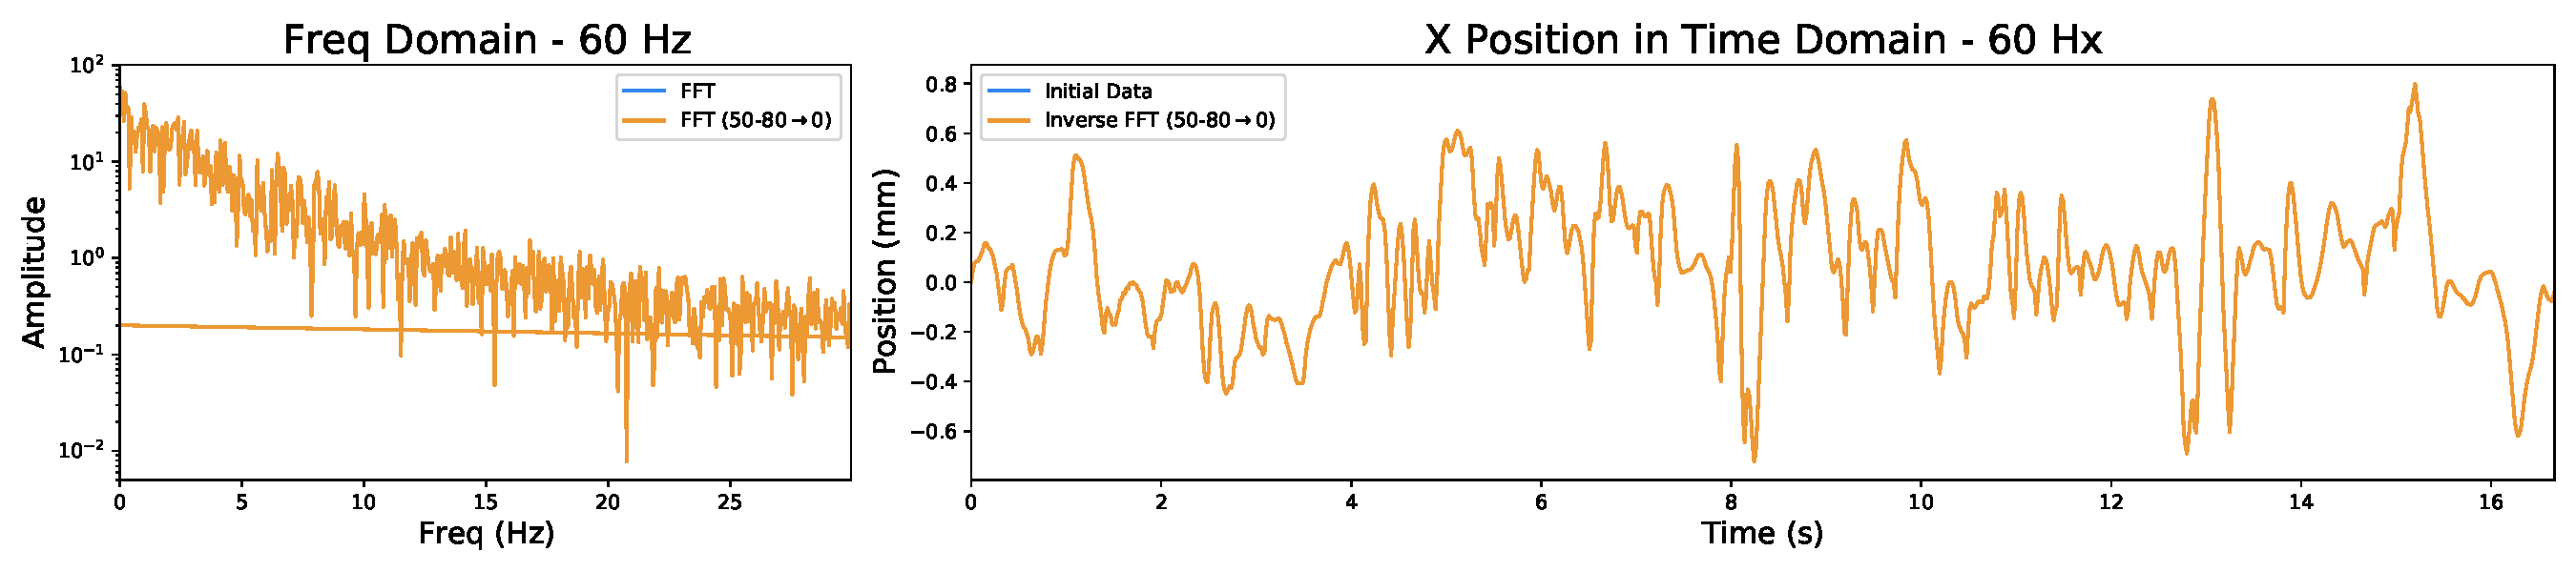
\includegraphics[width=\textwidth]{data_33_x_pos.pdf}
	\caption{}
    \label{fig:33_x_pos}
    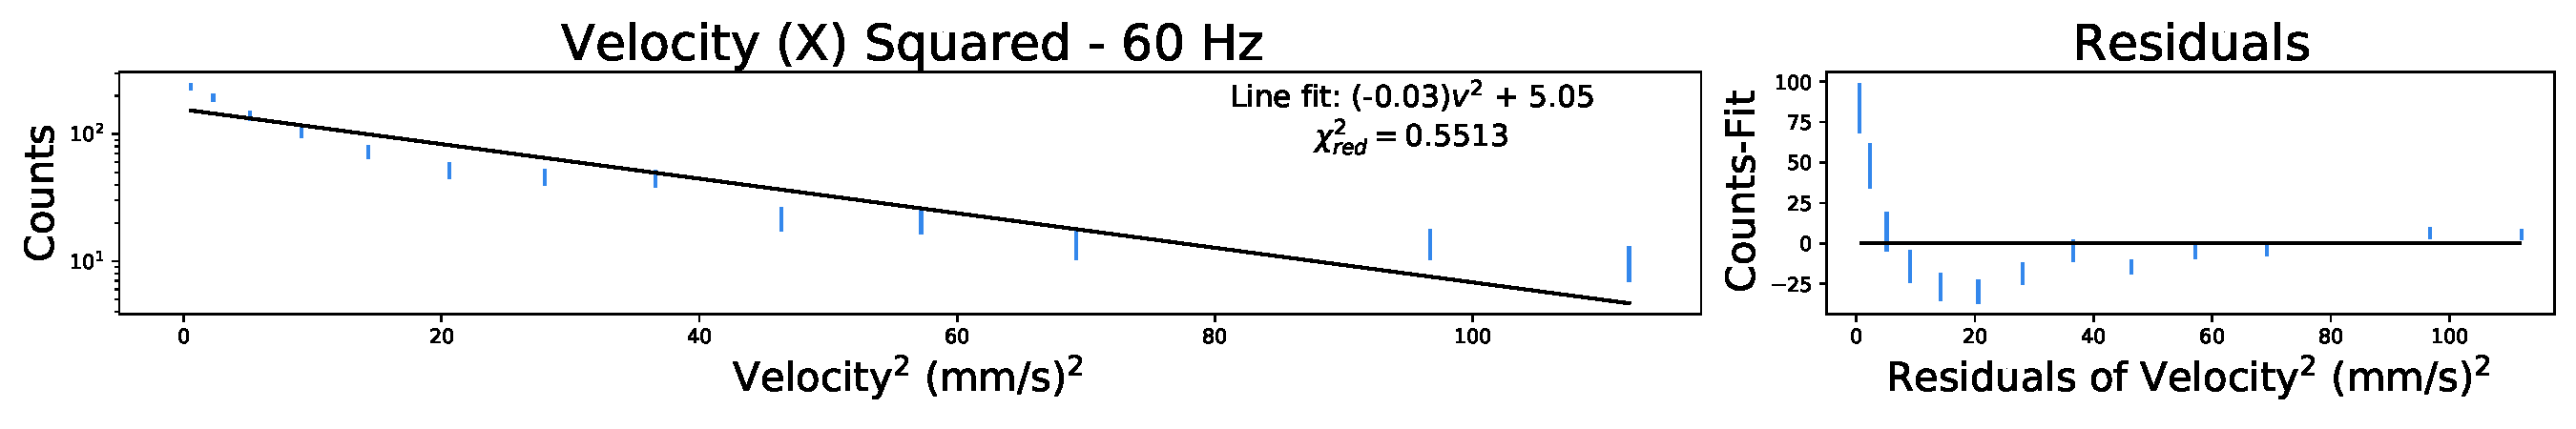
\includegraphics[width=\textwidth]{data_33_x_vel.pdf}
	\caption{}
    \label{fig:33_x_vel}
\end{figure}

\begin{figure}[ht]
\centering
    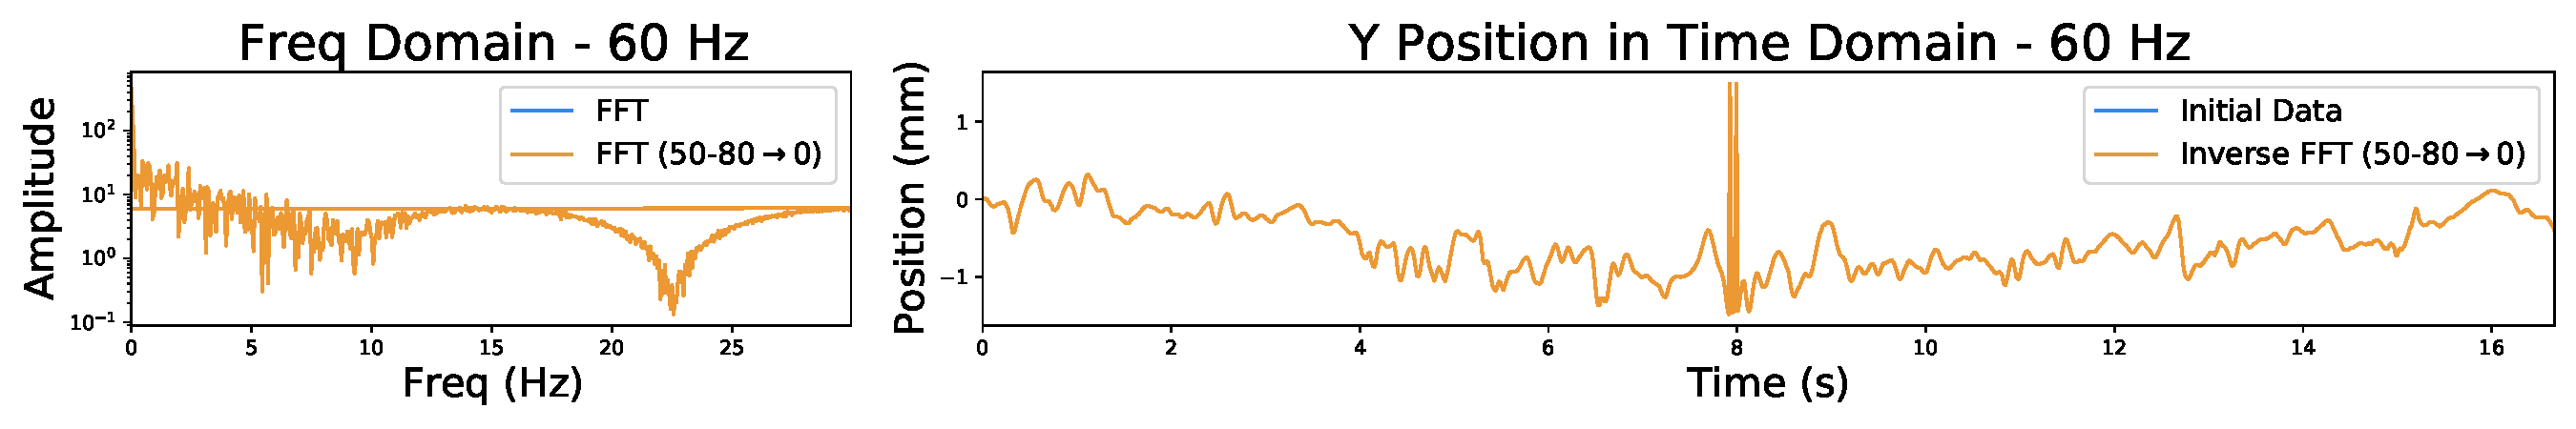
\includegraphics[width=\textwidth]{data_33_y_pos.pdf}
	\caption{}
    \label{fig:33_y_pos}
    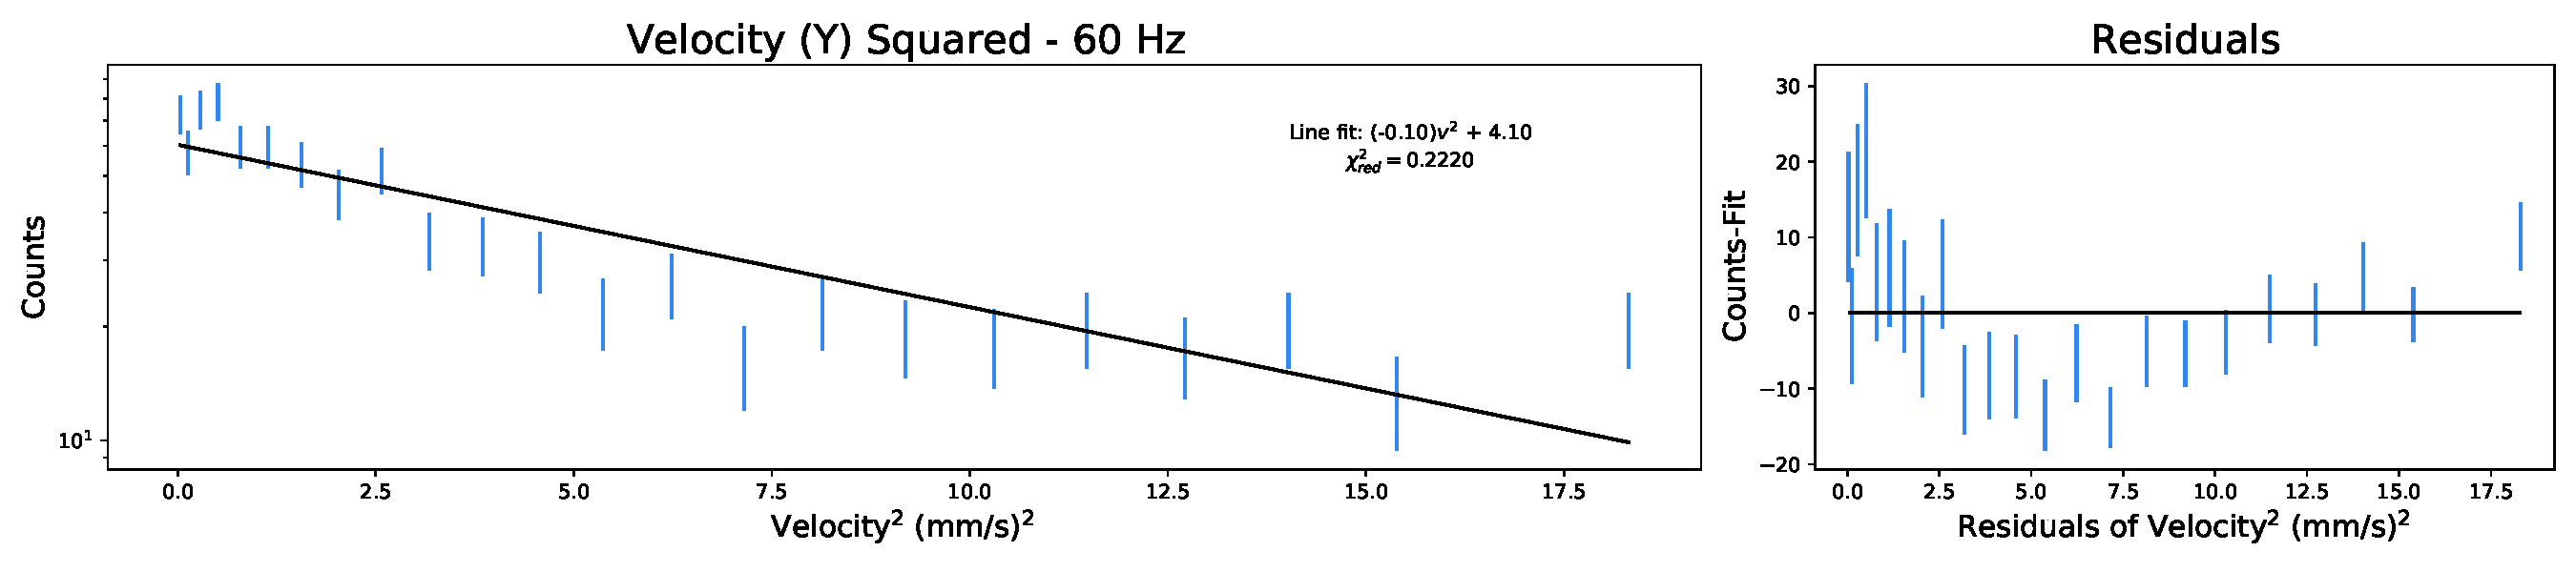
\includegraphics[width=\textwidth]{data_33_y_vel.pdf}
	\caption{}
    \label{fig:33_y_vel}
\end{figure}

\begin{figure}[ht]
\centering
    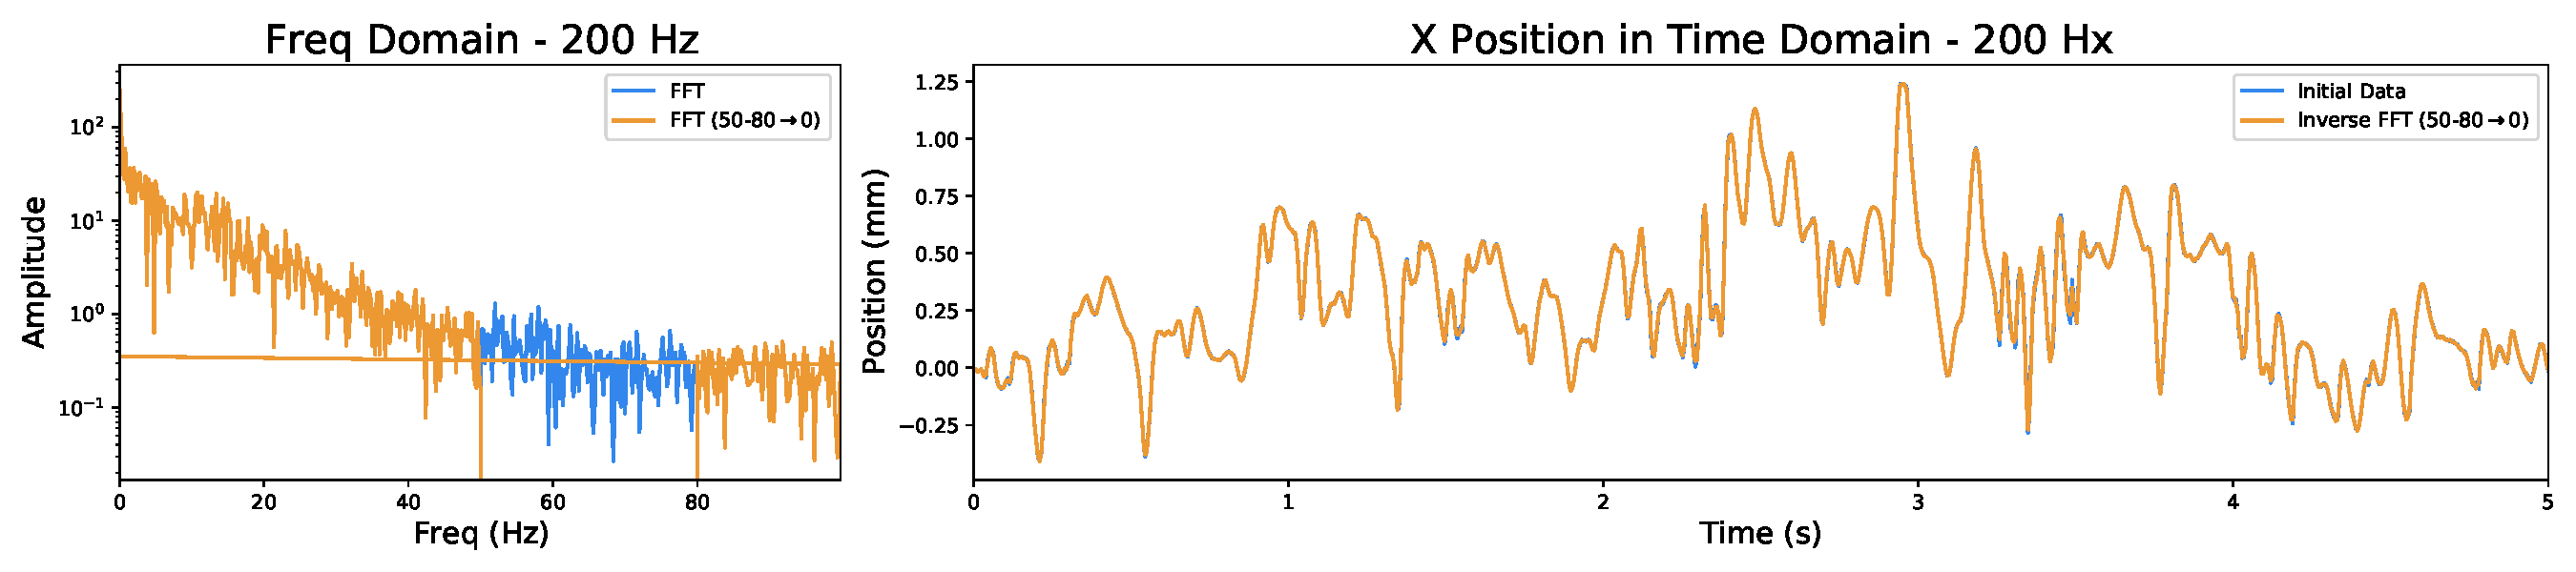
\includegraphics[width=\textwidth]{data_36_x_pos.pdf}
	\caption{}
    \label{fig:36_x_pos}
    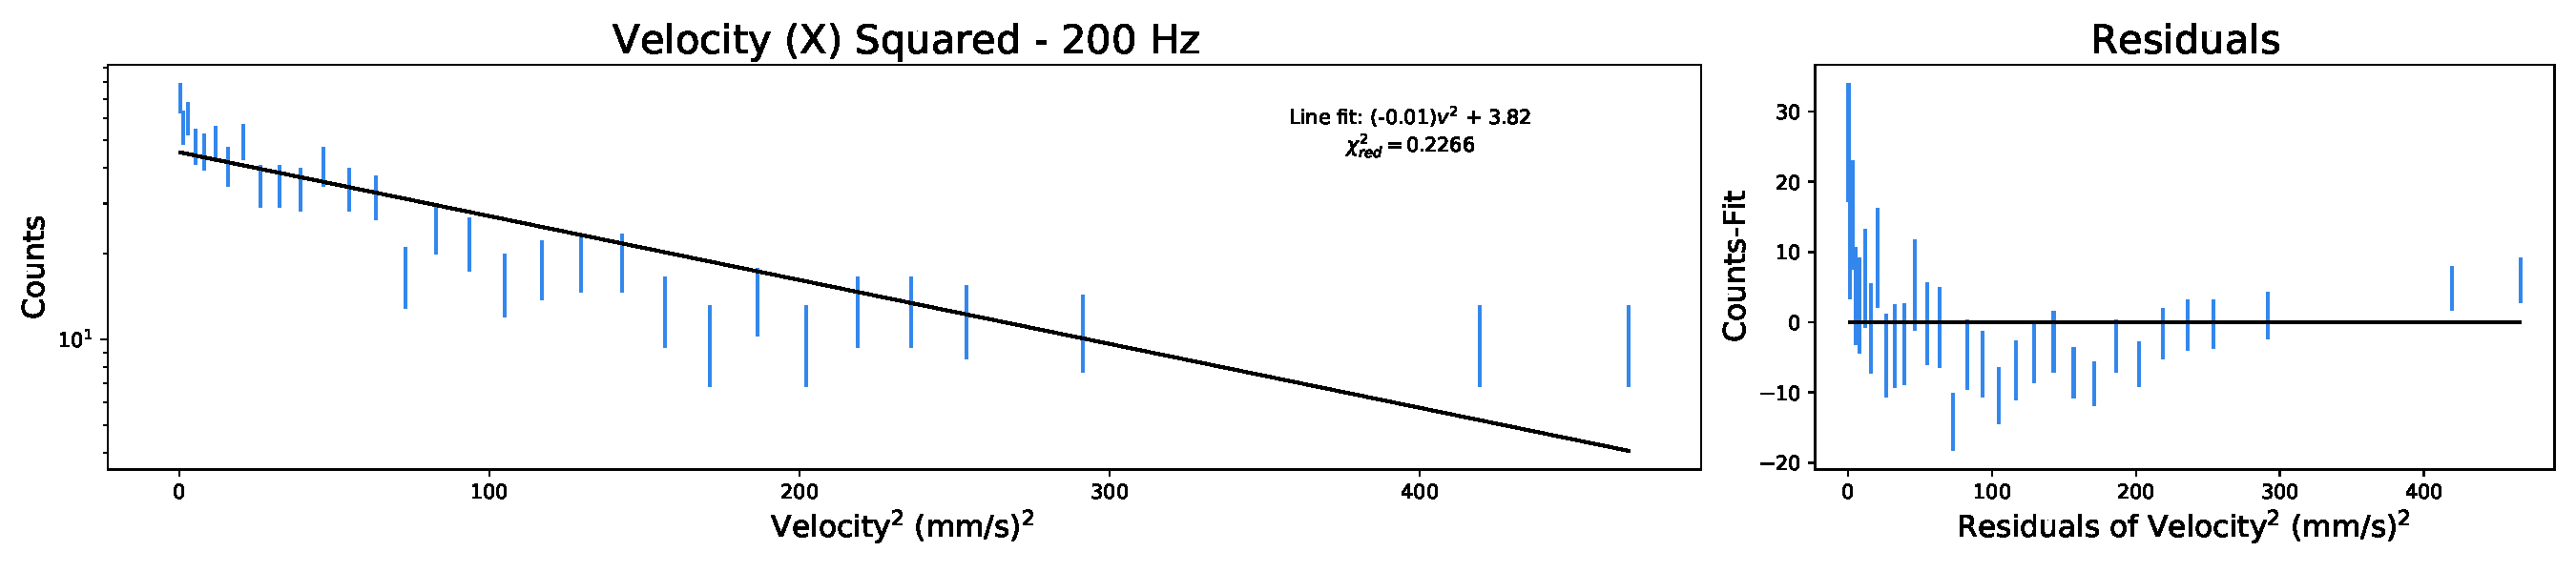
\includegraphics[width=\textwidth]{data_36_x_vel.pdf}
	\caption{}
    \label{fig:36_x_vel}
\end{figure}

\subsection{Analyzing Motion}
%% Give the analysis of motion, x and y
\begin{figure}[ht]
\centering
    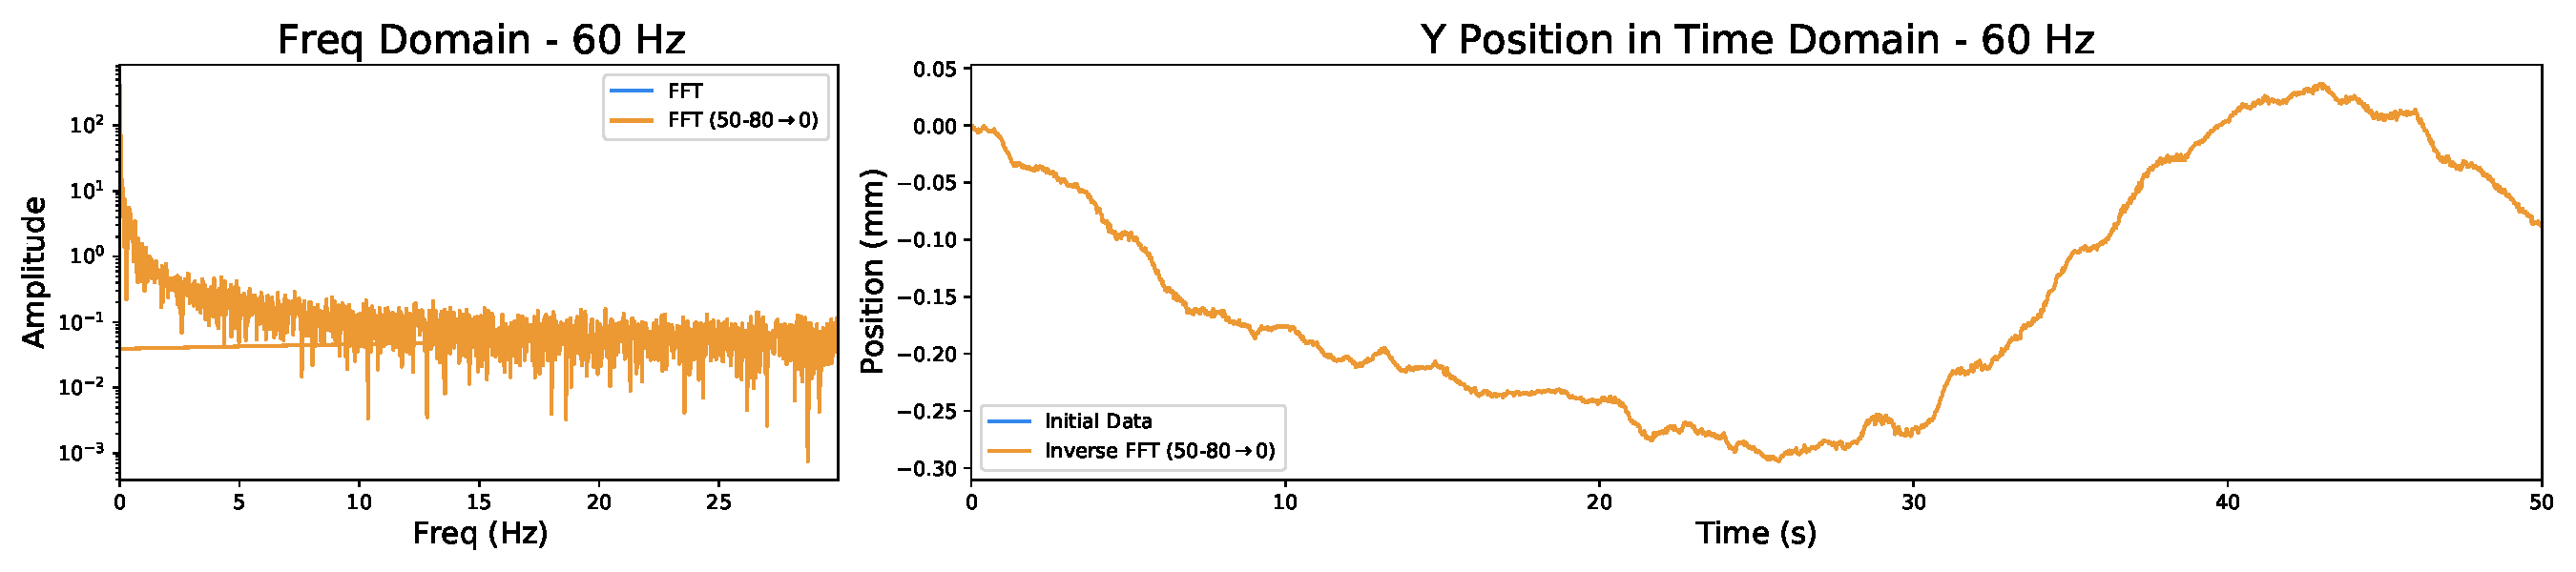
\includegraphics[width=\textwidth]{data_01_y_pos.pdf}
	\caption{}
    \label{fig:01_y_pos}
    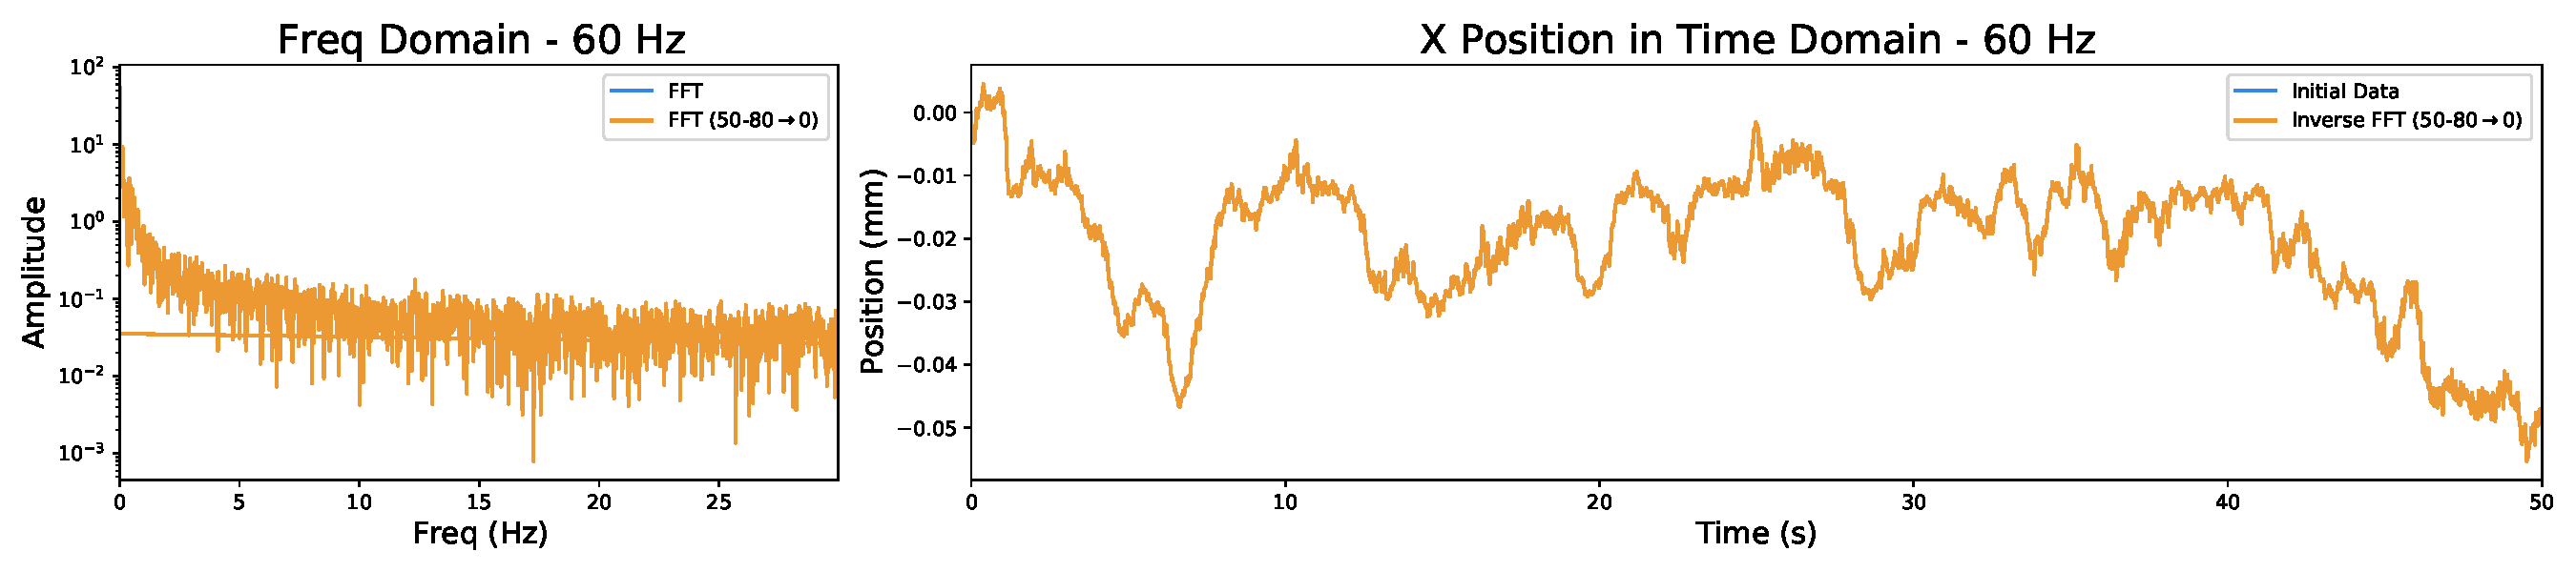
\includegraphics[width=\textwidth]{data_01_x_pos.pdf}
	\caption{}
    \label{fig:01_x_pos}
\end{figure}

\begin{figure}[ht]
\centering
    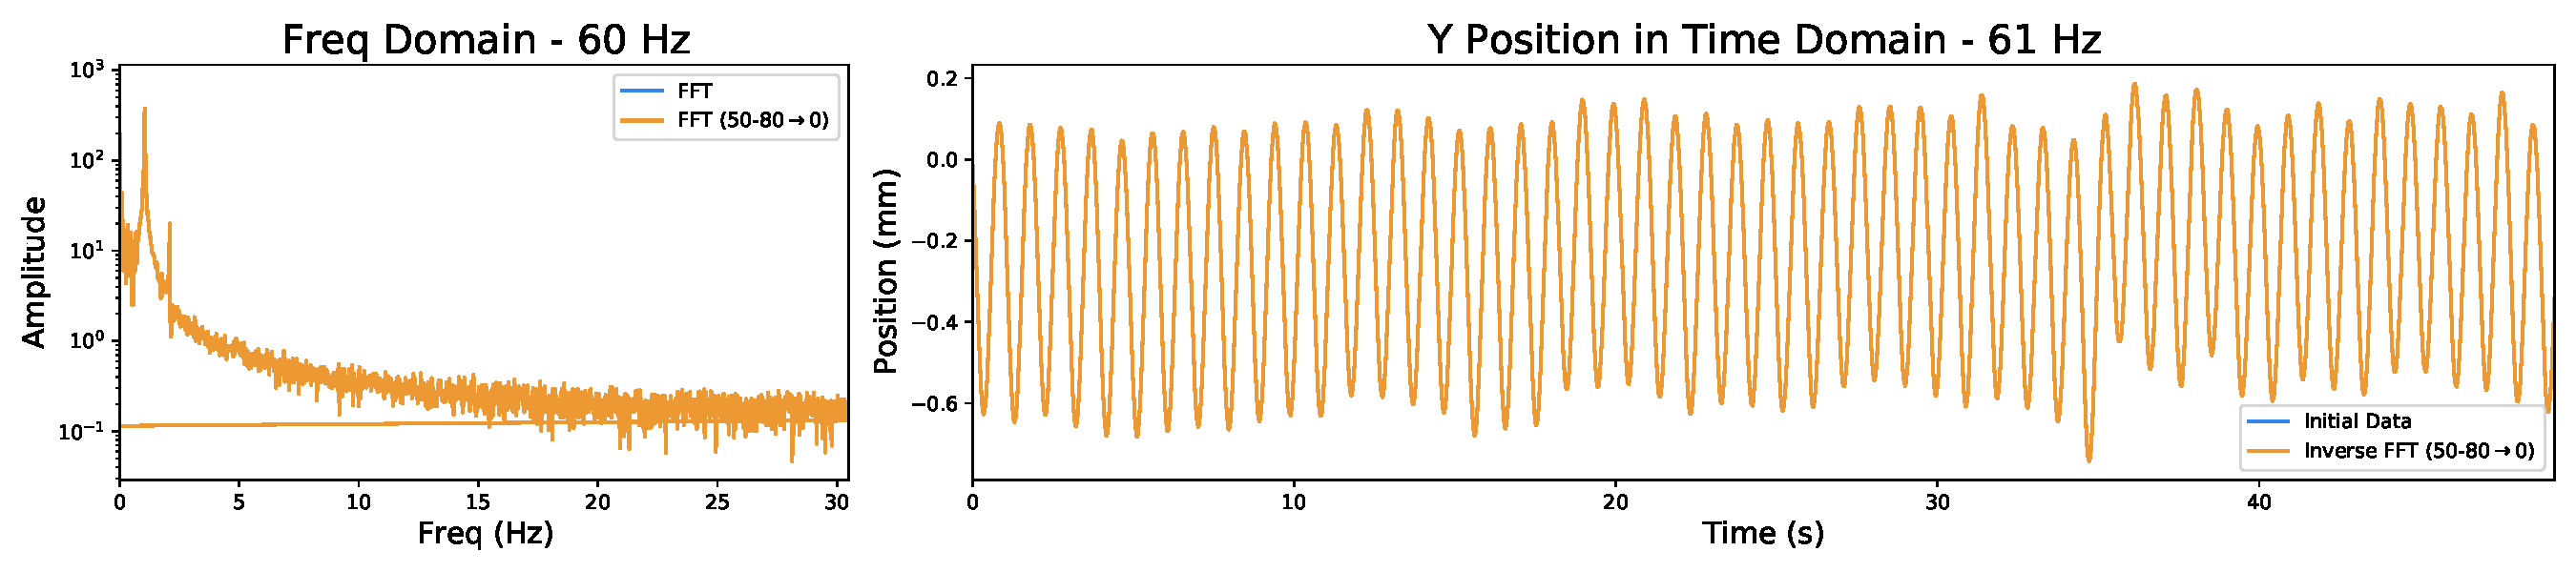
\includegraphics[width=\textwidth]{data_03_y_pos.pdf}
	\caption{}
    \label{fig:03_y_pos}
    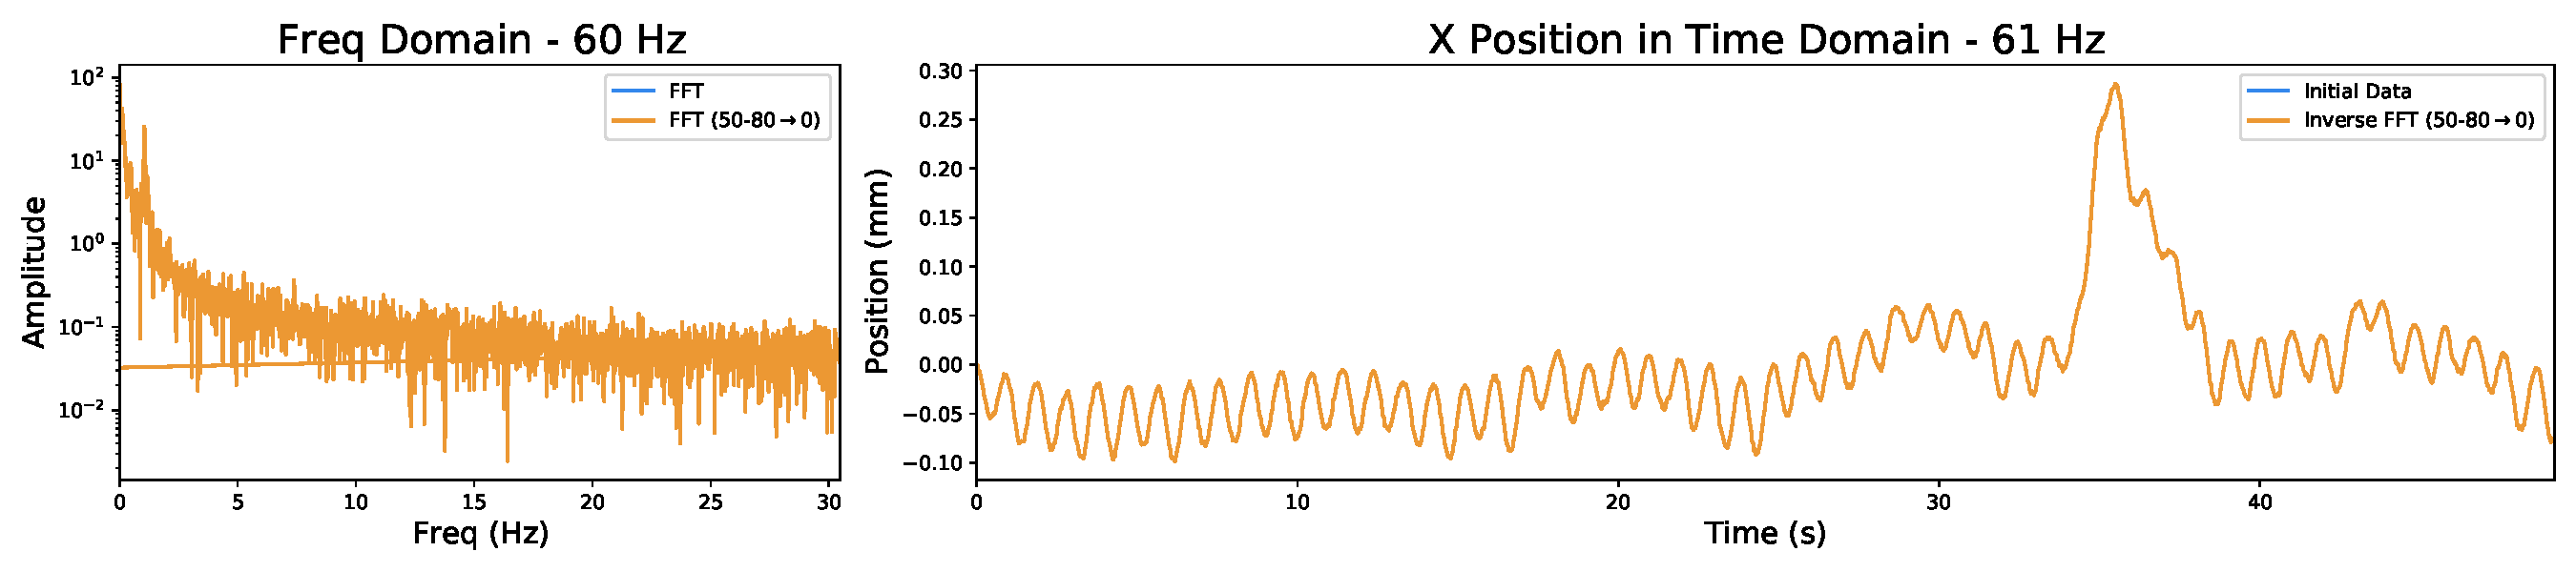
\includegraphics[width=\textwidth]{data_03_x_pos.pdf}
	\caption{}
    \label{fig:03_x_pos}
\end{figure}

\begin{figure}[ht]
\centering
    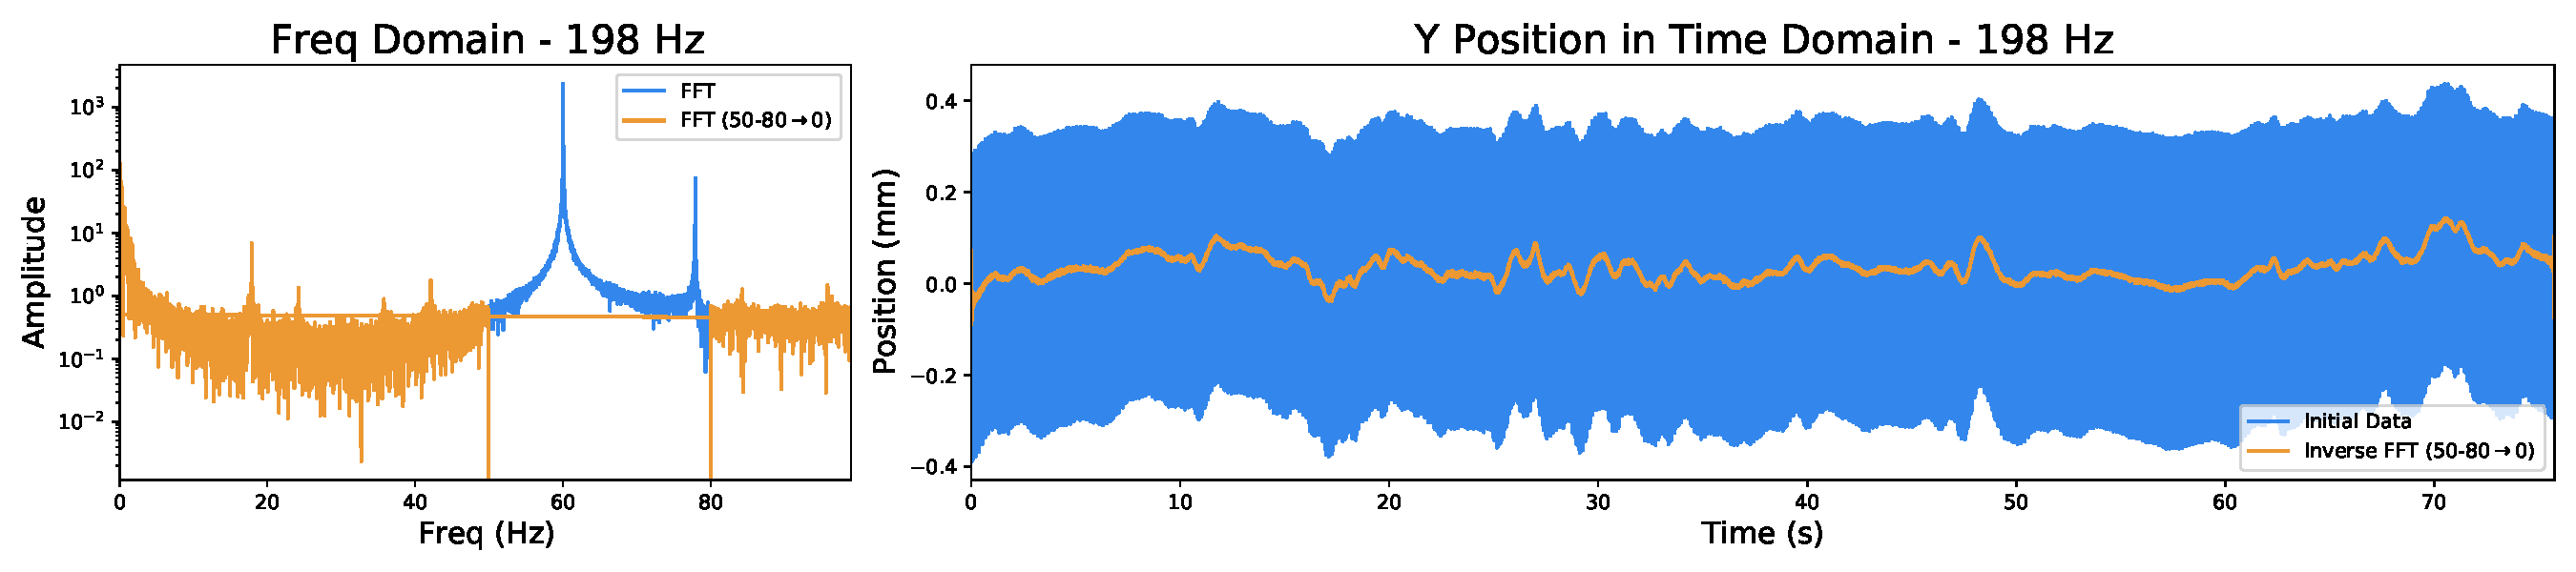
\includegraphics[width=\textwidth]{data_04_y_pos.pdf}
	\caption{}
    \label{fig:04_y_pos}
    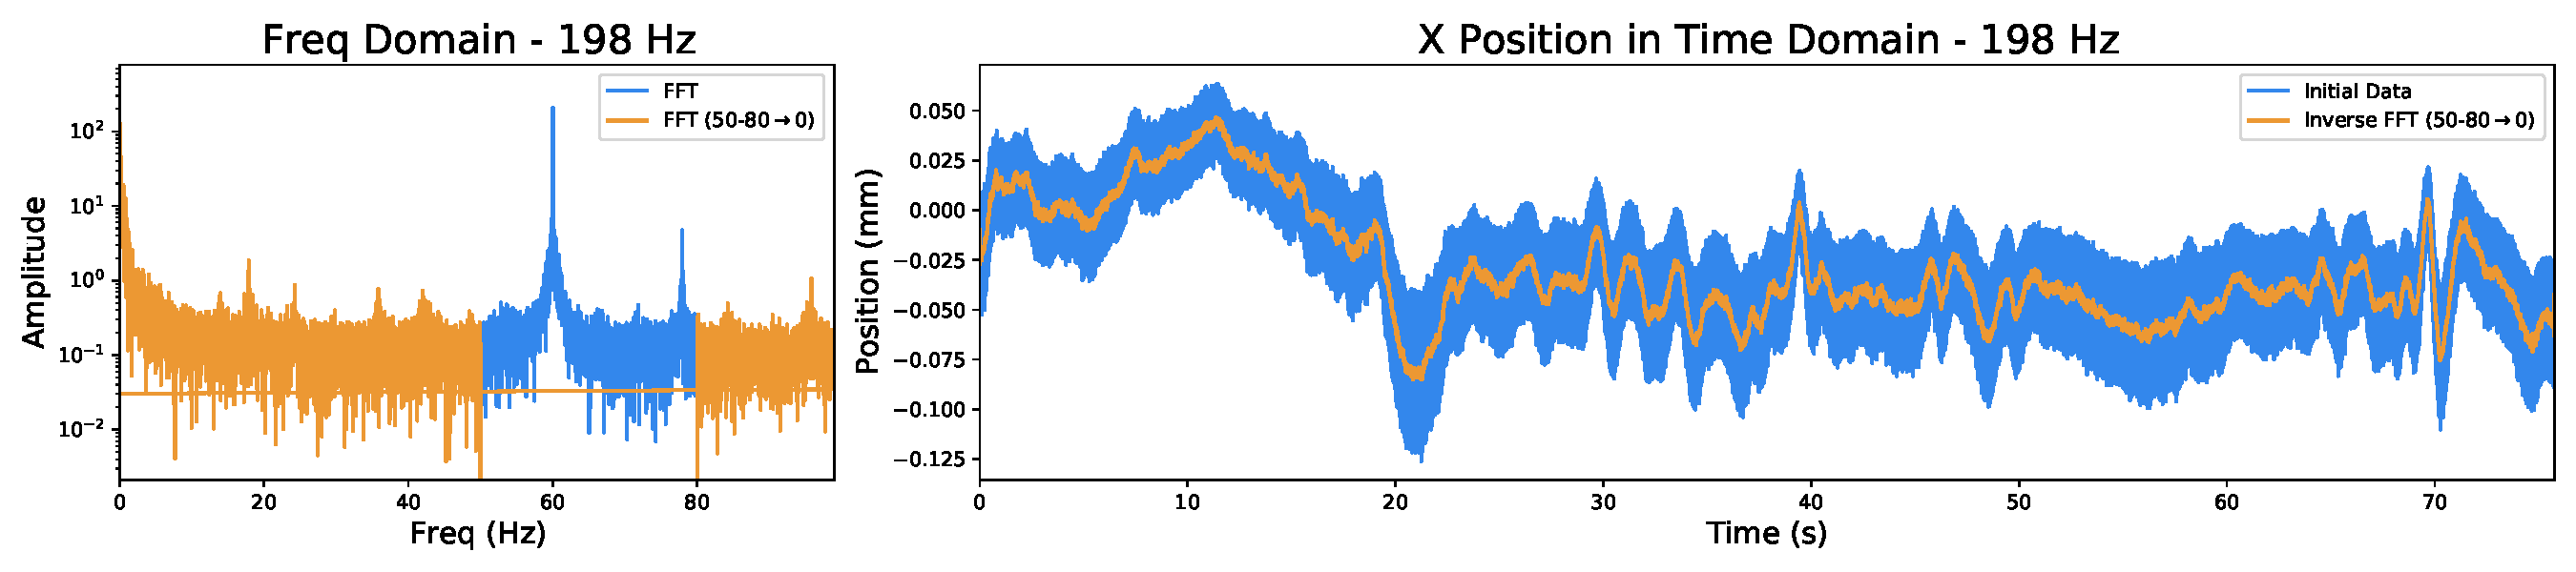
\includegraphics[width=\textwidth]{data_04_x_pos.pdf}
	\caption{}
    \label{fig:04_x_pos}
\end{figure}


\subsection{Transient Response}
%% Give the transient response

\begin{figure}[ht]
\centering
    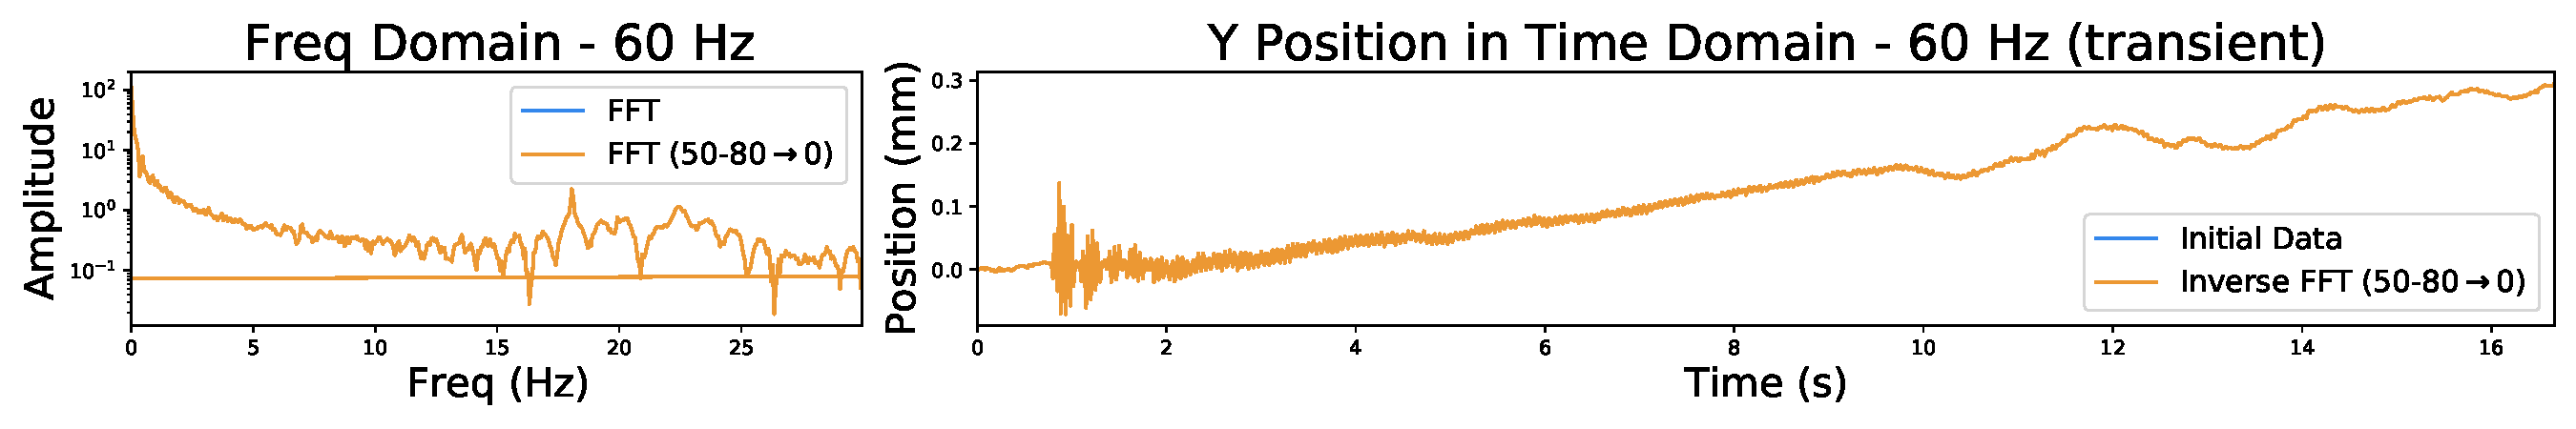
\includegraphics[width=\textwidth]{data_02_y_pos.pdf}
	\caption{}
    \label{fig:02_y_pos}
    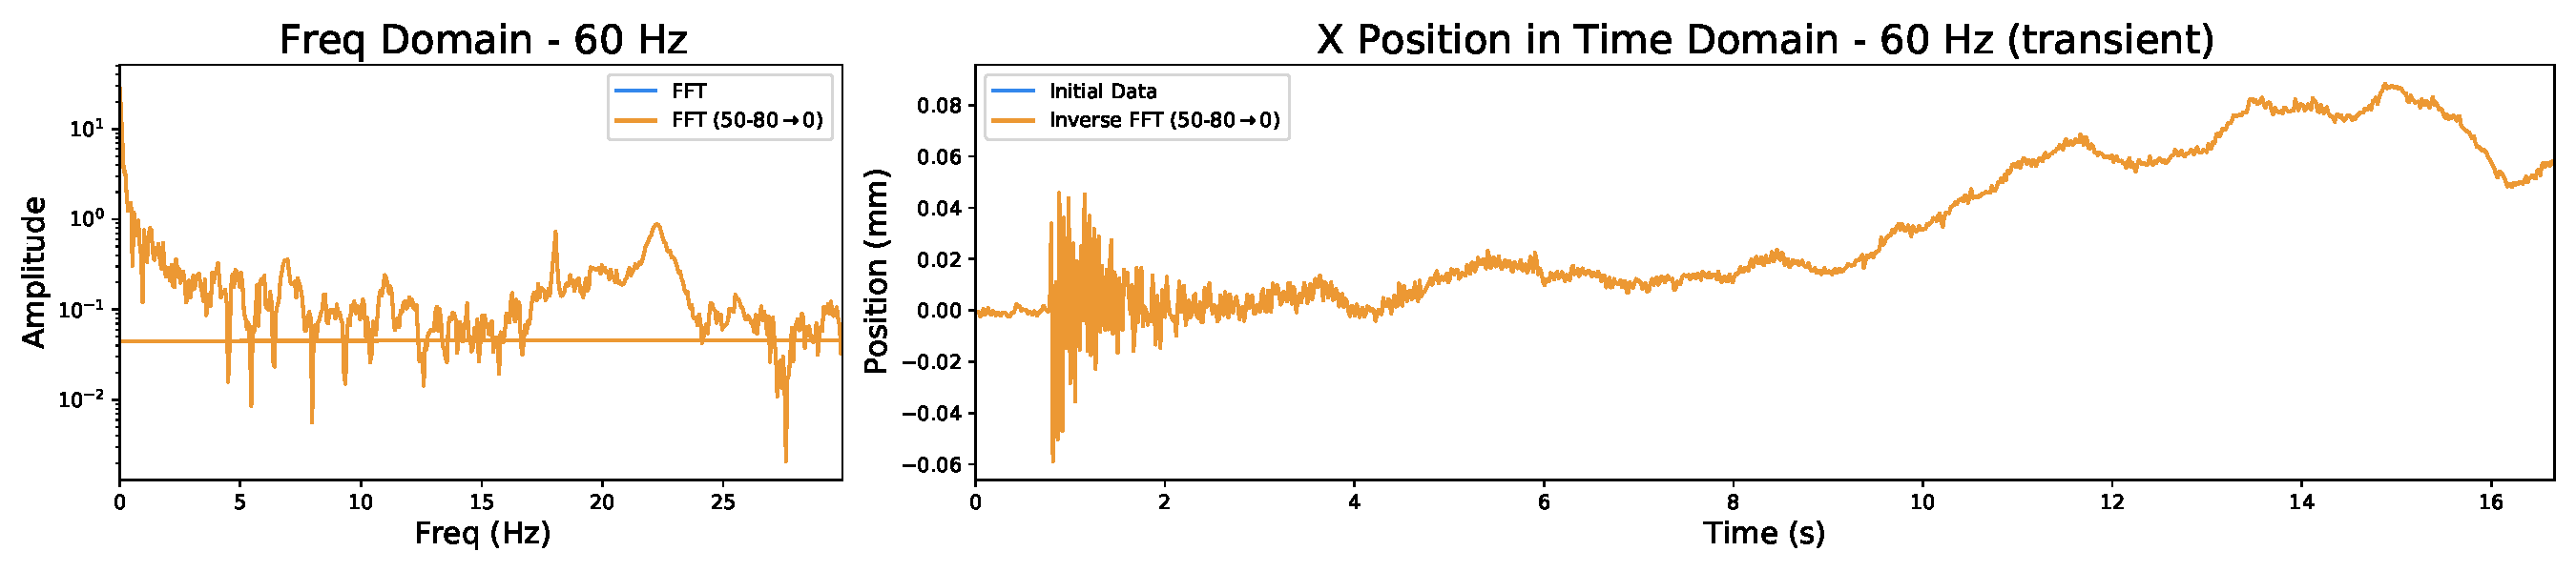
\includegraphics[width=\textwidth]{data_02_x_pos.pdf}
	\caption{}
    \label{fig:02_x_pos}
\end{figure}

\begin{figure}[ht]
\centering
    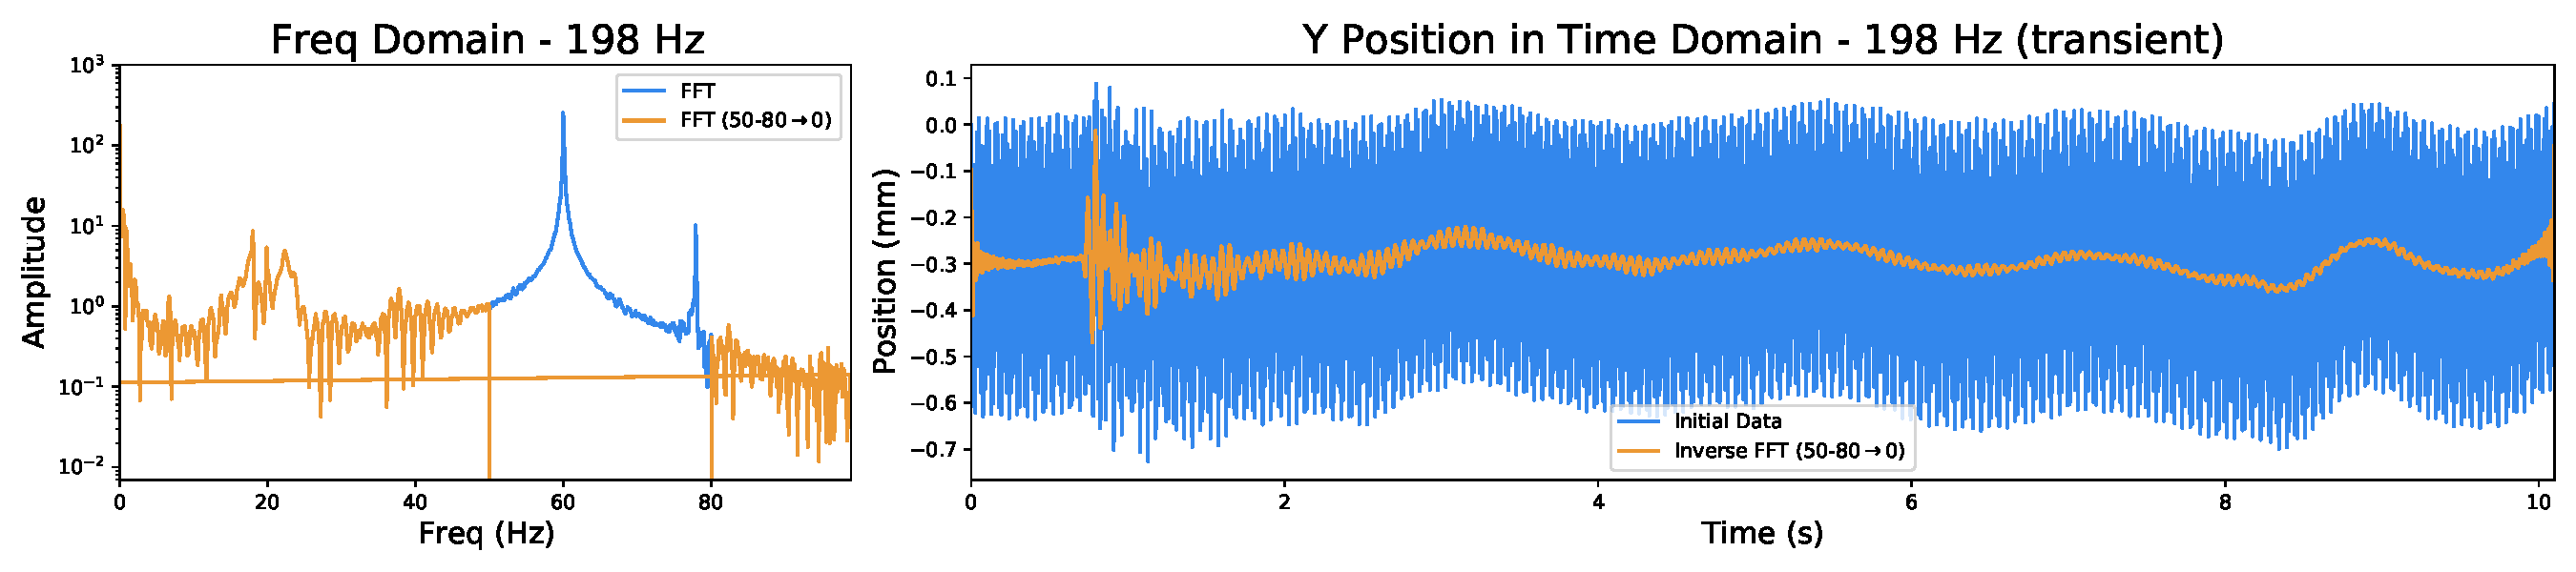
\includegraphics[width=\textwidth]{data_05_y_pos.pdf}
	\caption{}
    \label{fig:05_y_pos}
    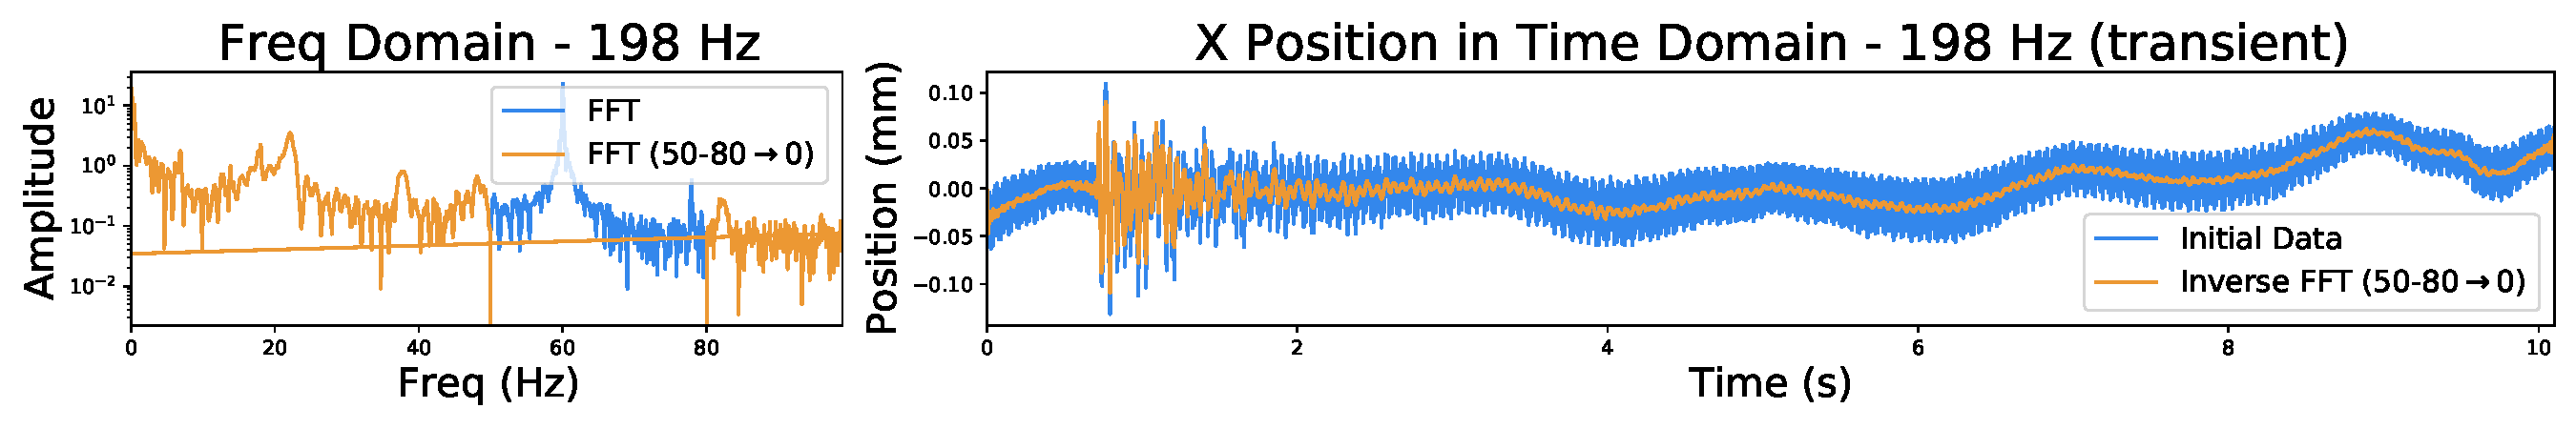
\includegraphics[width=\textwidth]{data_05_x_pos.pdf}
	\caption{}
    \label{fig:05_x_pos}
\end{figure}

\subsection{Analyzing Velocity}
%% Give the analysis of velocity
\begin{figure}[ht]
\centering
    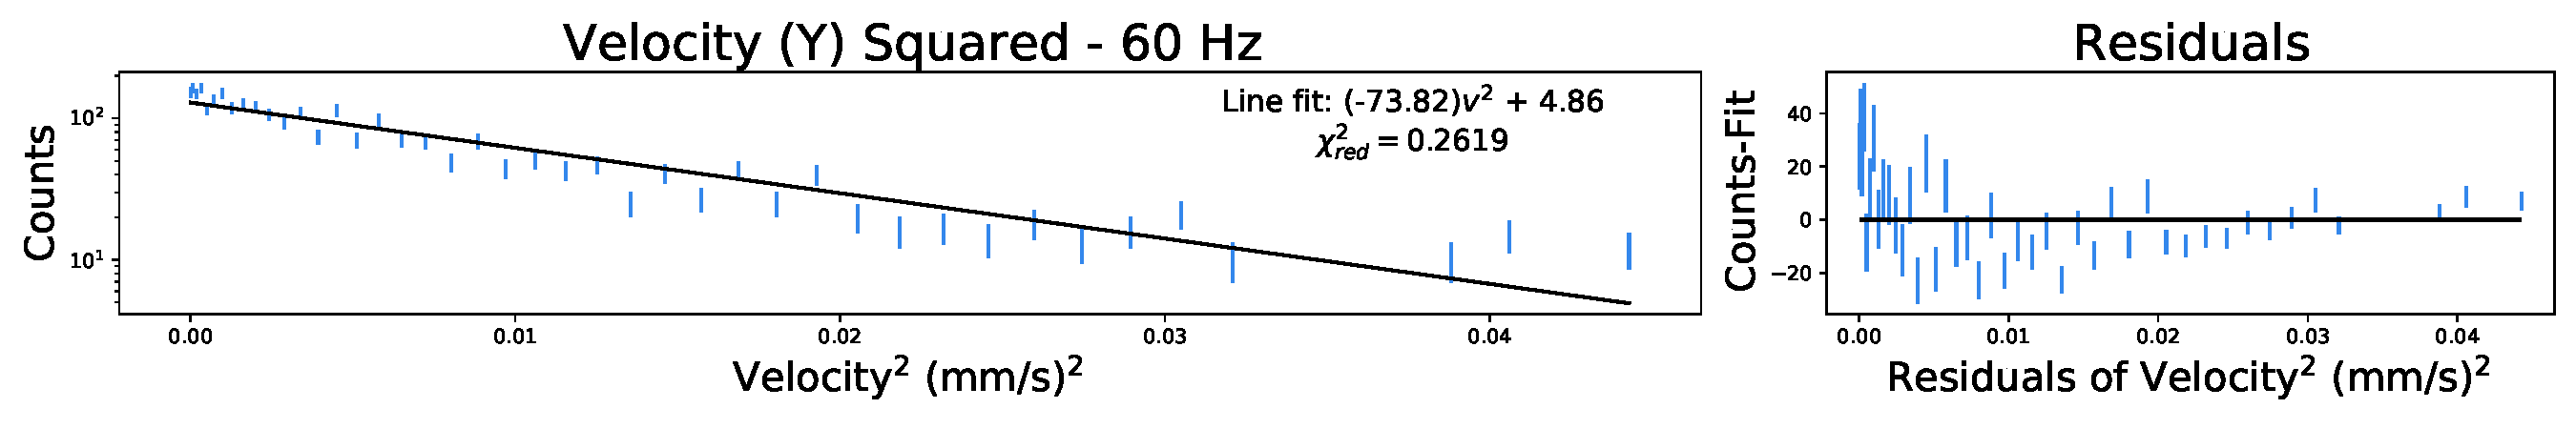
\includegraphics[width=\textwidth]{data_01_y_vel.pdf}
	\caption{}
    \label{fig:01_y_vel}
    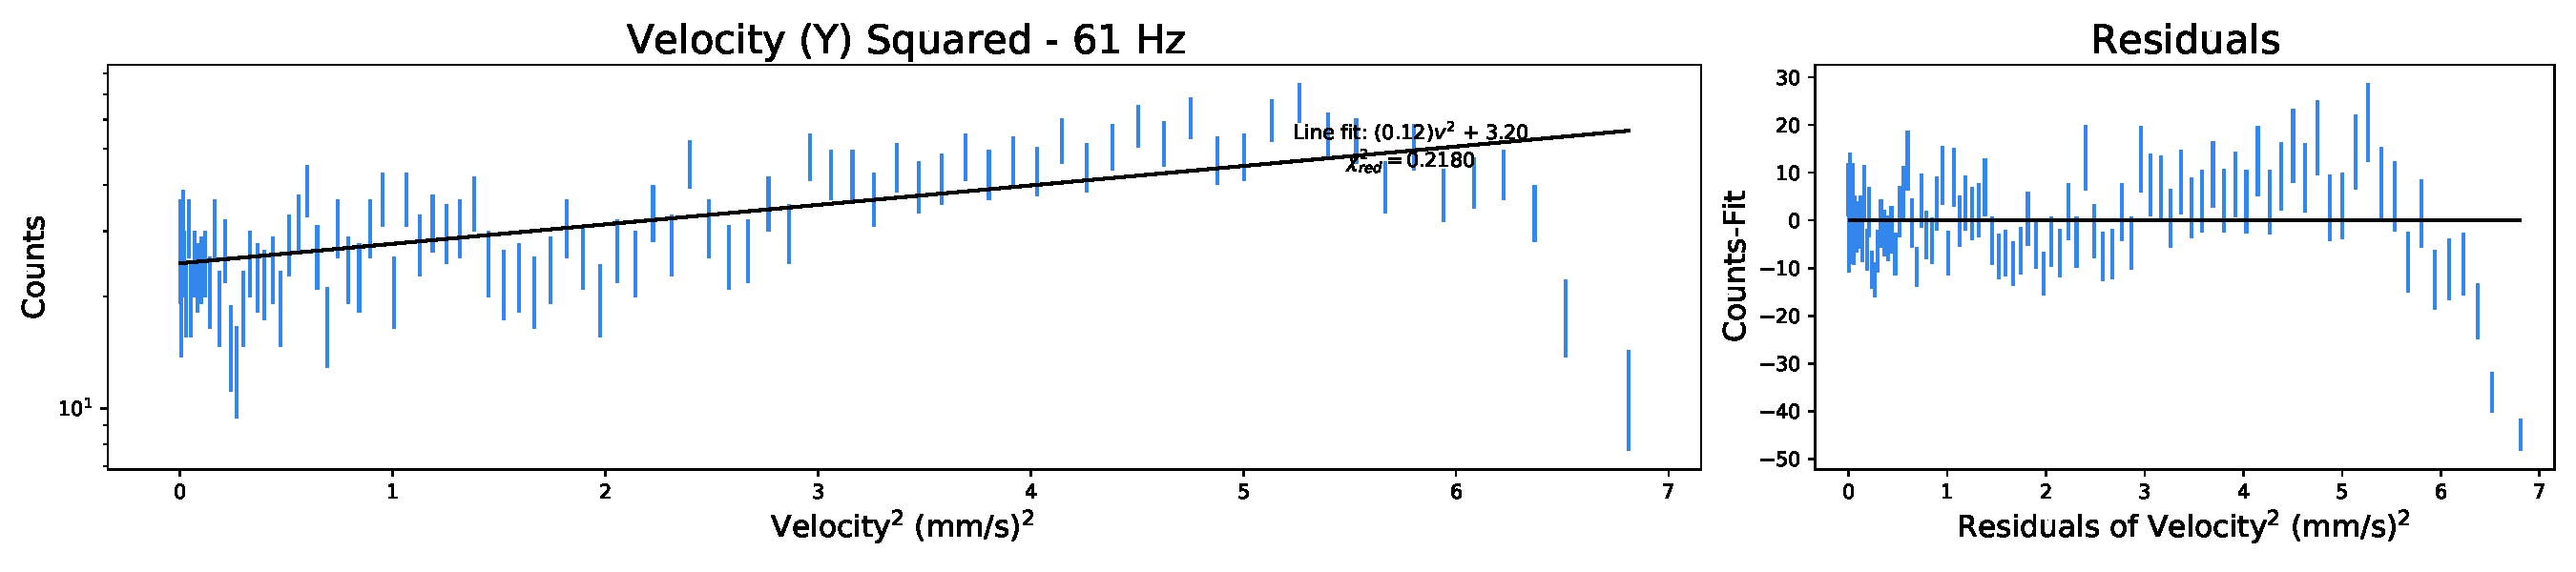
\includegraphics[width=\textwidth]{data_03_y_vel.pdf}
	\caption{}
    \label{fig:03_y_vel}
    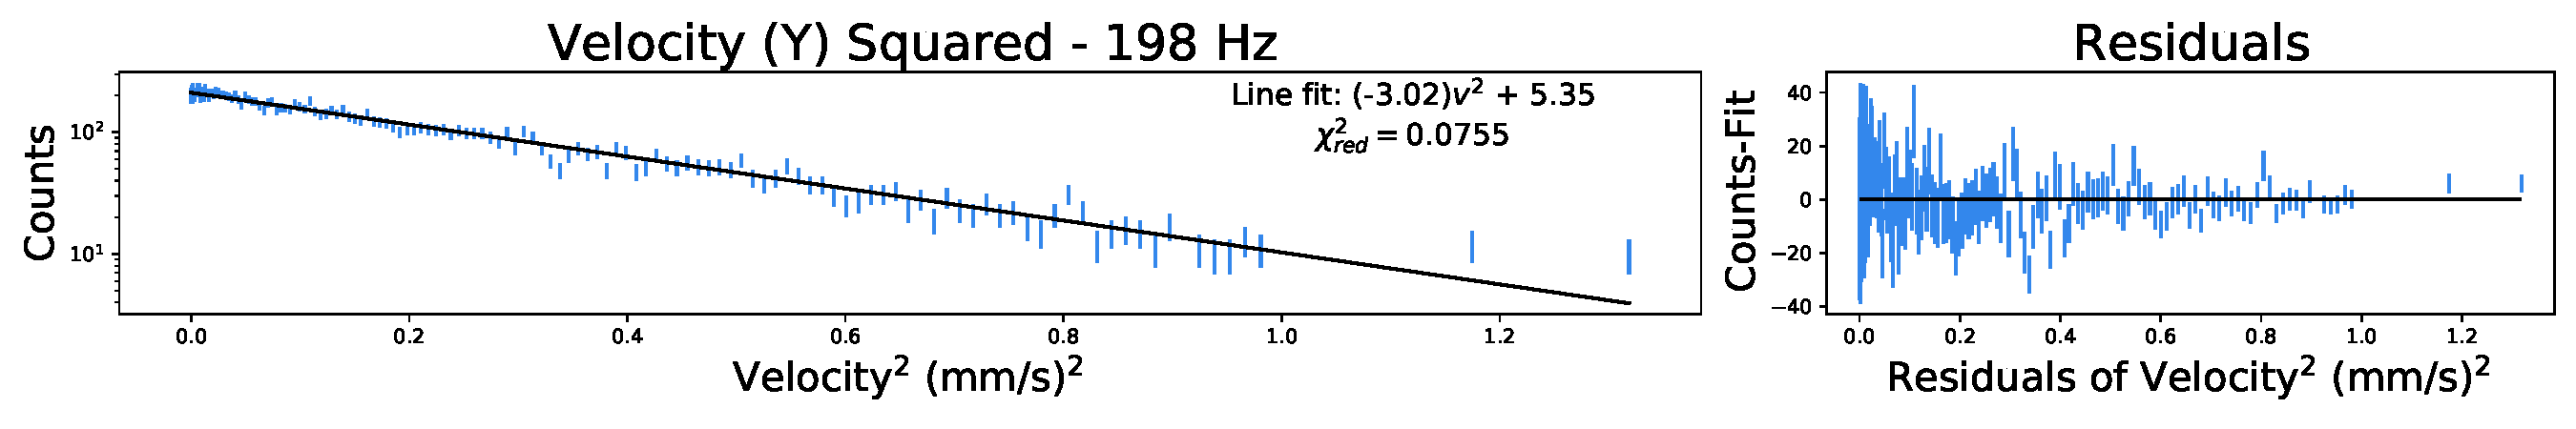
\includegraphics[width=\textwidth]{data_04_y_vel.pdf}
	\caption{}
    \label{fig:04_y_vel}
\end{figure}


\begin{figure}[ht]
\centering
    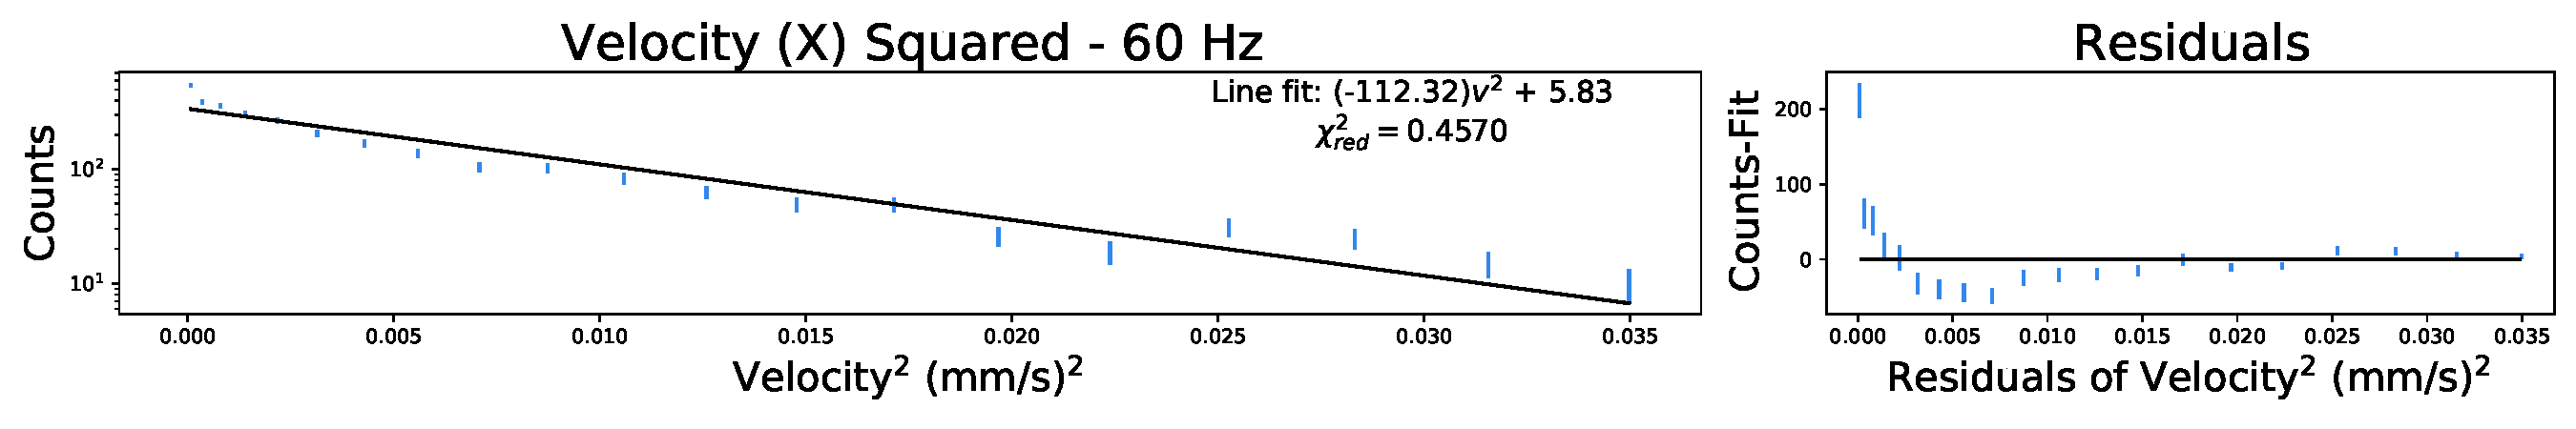
\includegraphics[width=\textwidth]{data_01_x_vel.pdf}
	\caption{}
    \label{fig:01_x_vel}
    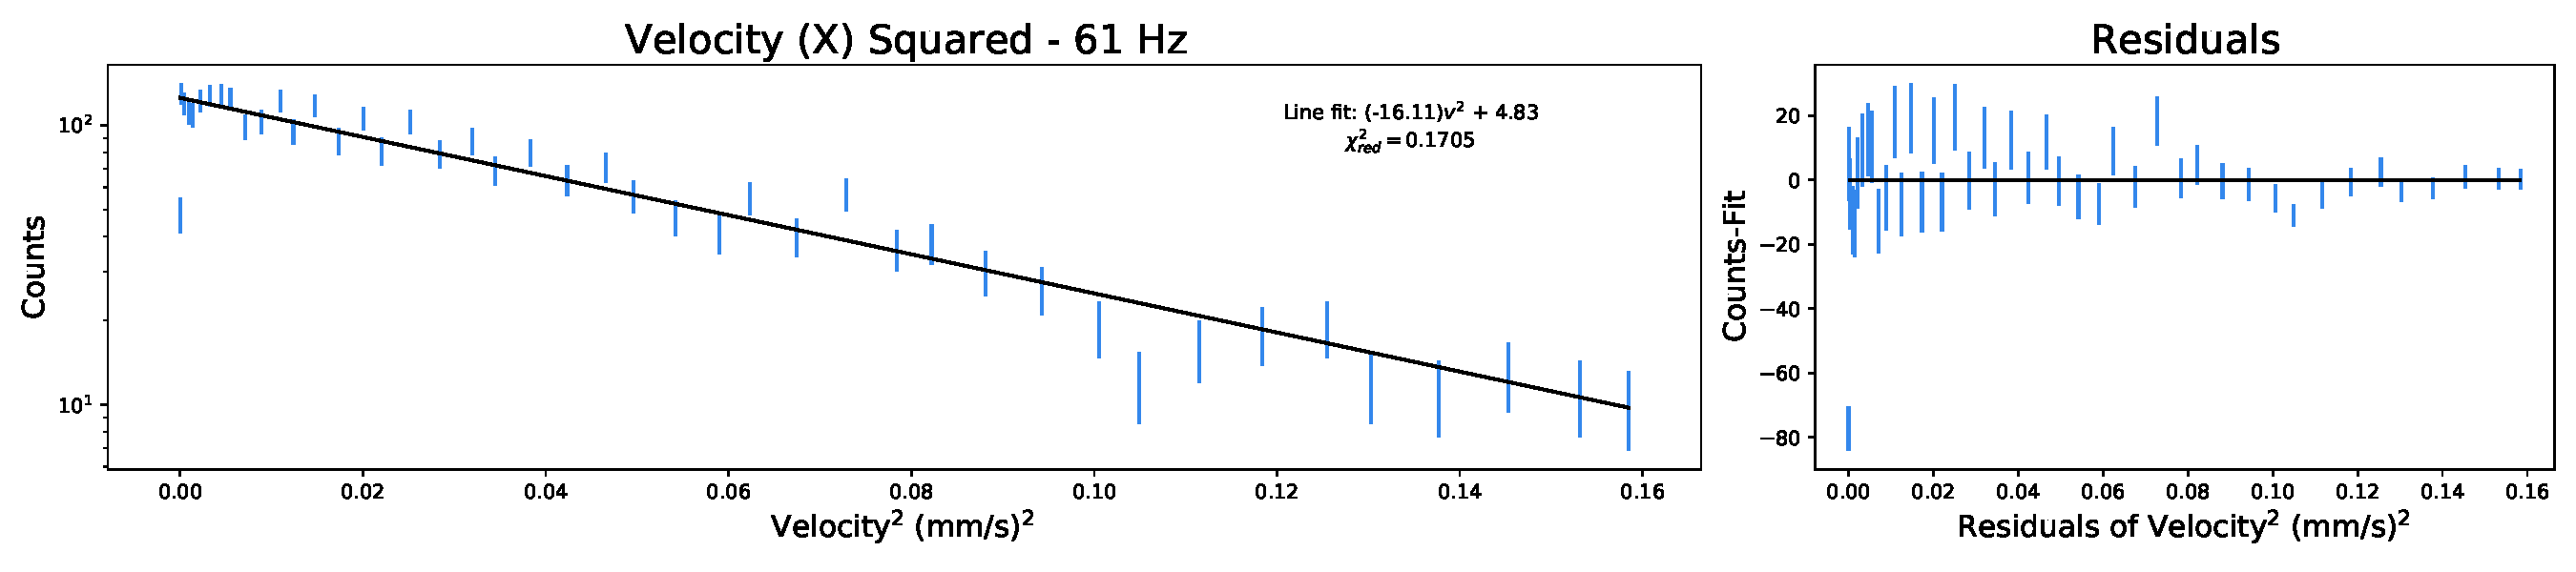
\includegraphics[width=\textwidth]{data_03_x_vel.pdf}
	\caption{}
    \label{fig:03_x_vel}
    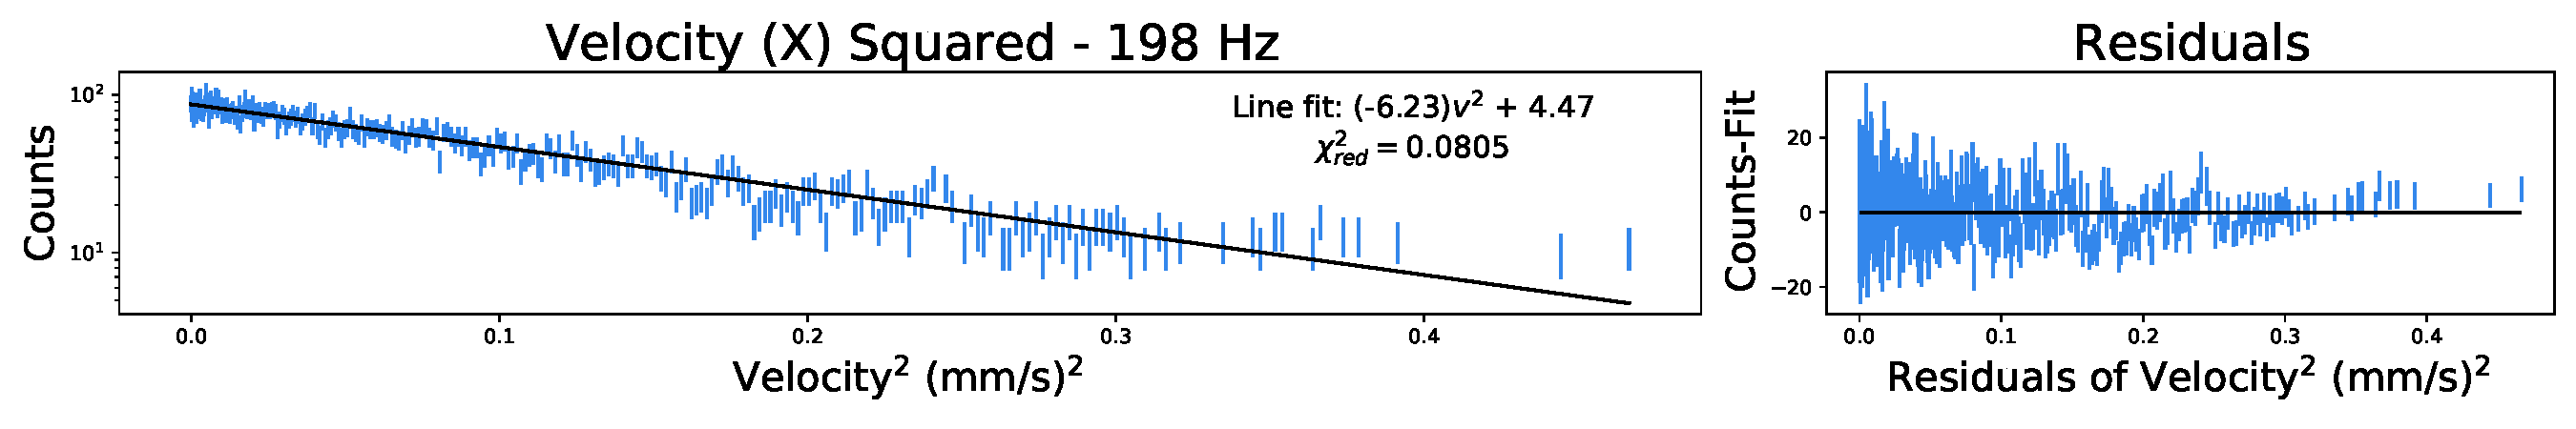
\includegraphics[width=\textwidth]{data_04_x_vel.pdf}
	\caption{}
    \label{fig:04_x_vel}
\end{figure}

\begin{figure}[ht]
\centering
    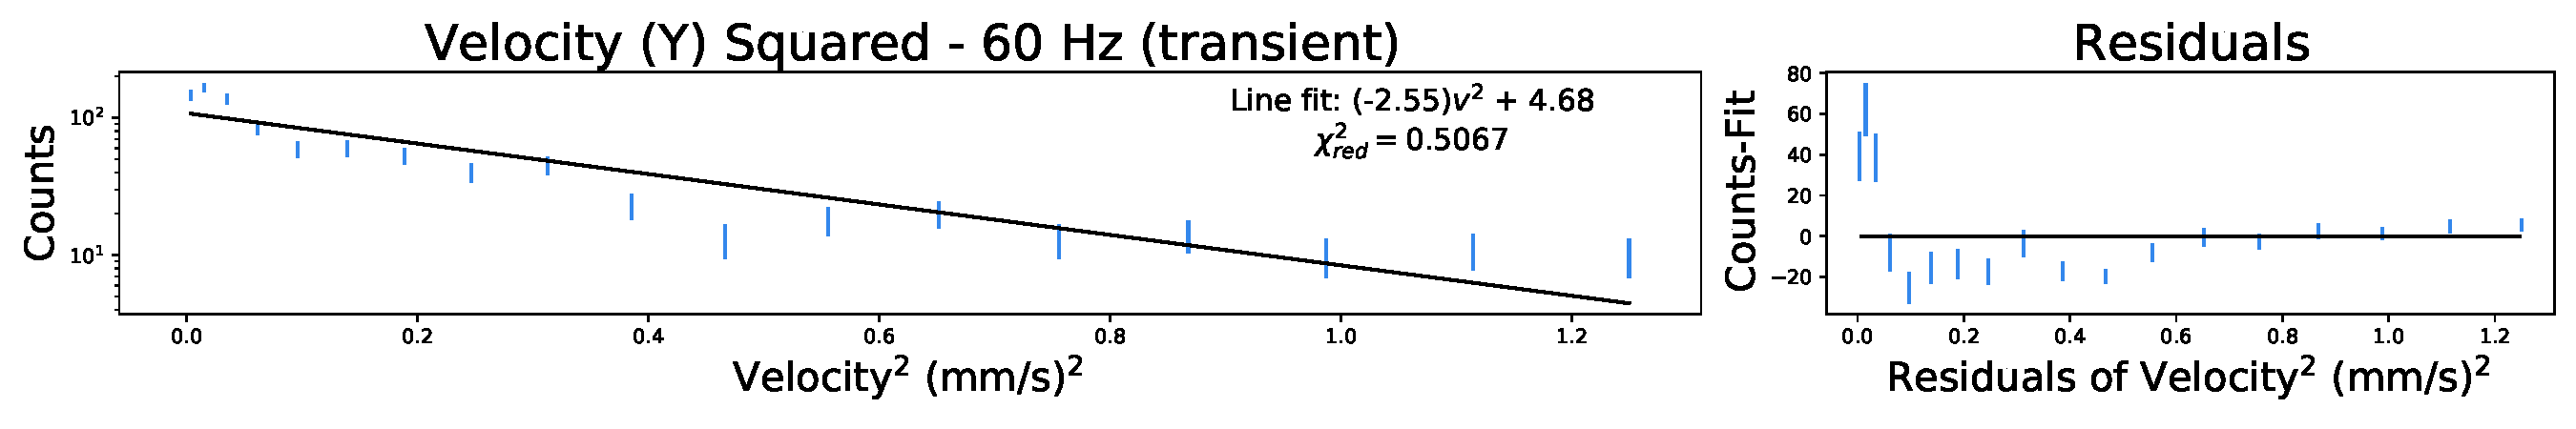
\includegraphics[width=\textwidth]{data_02_y_vel.pdf}
	\caption{}
    \label{fig:02_y_vel}
    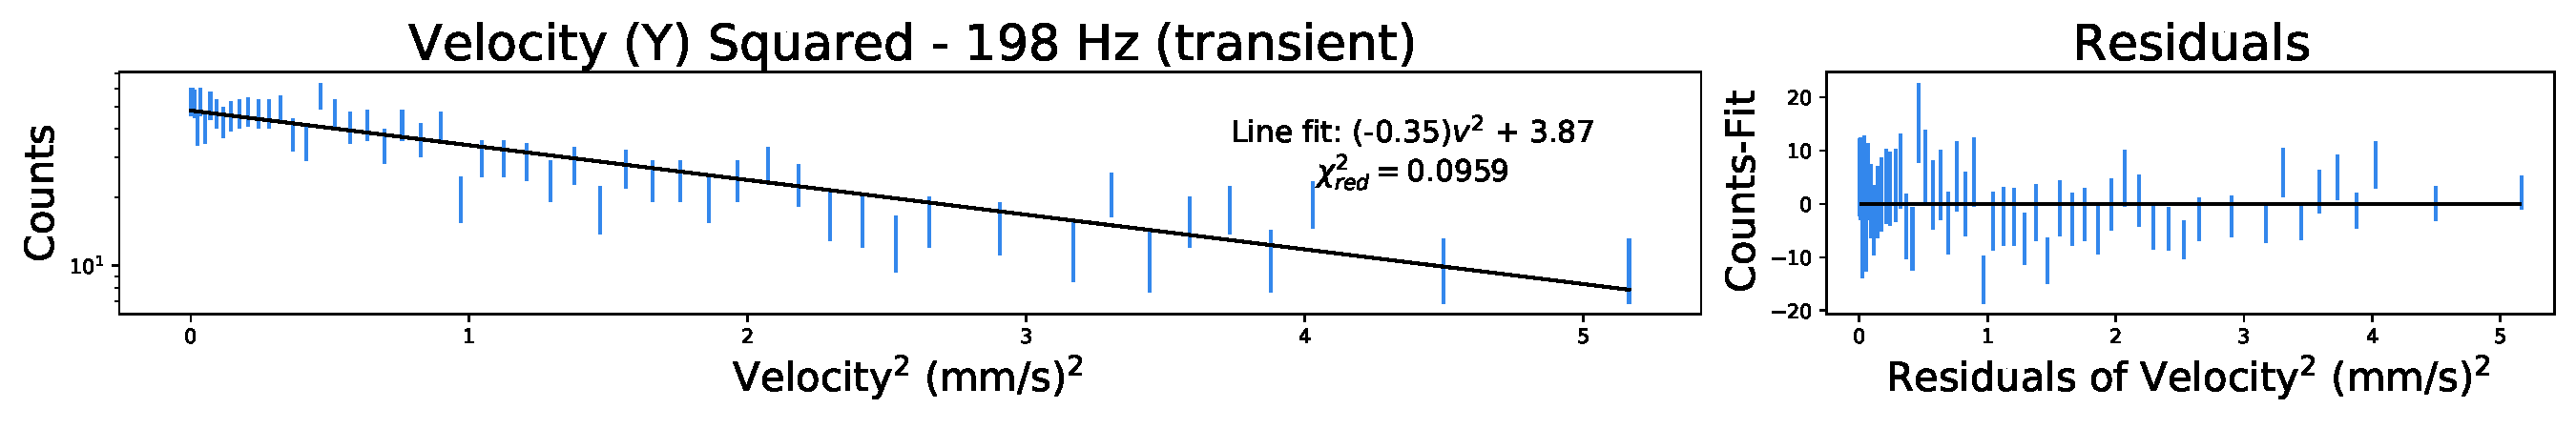
\includegraphics[width=\textwidth]{data_05_y_vel.pdf}
	\caption{}
    \label{fig:05_y_vel}
    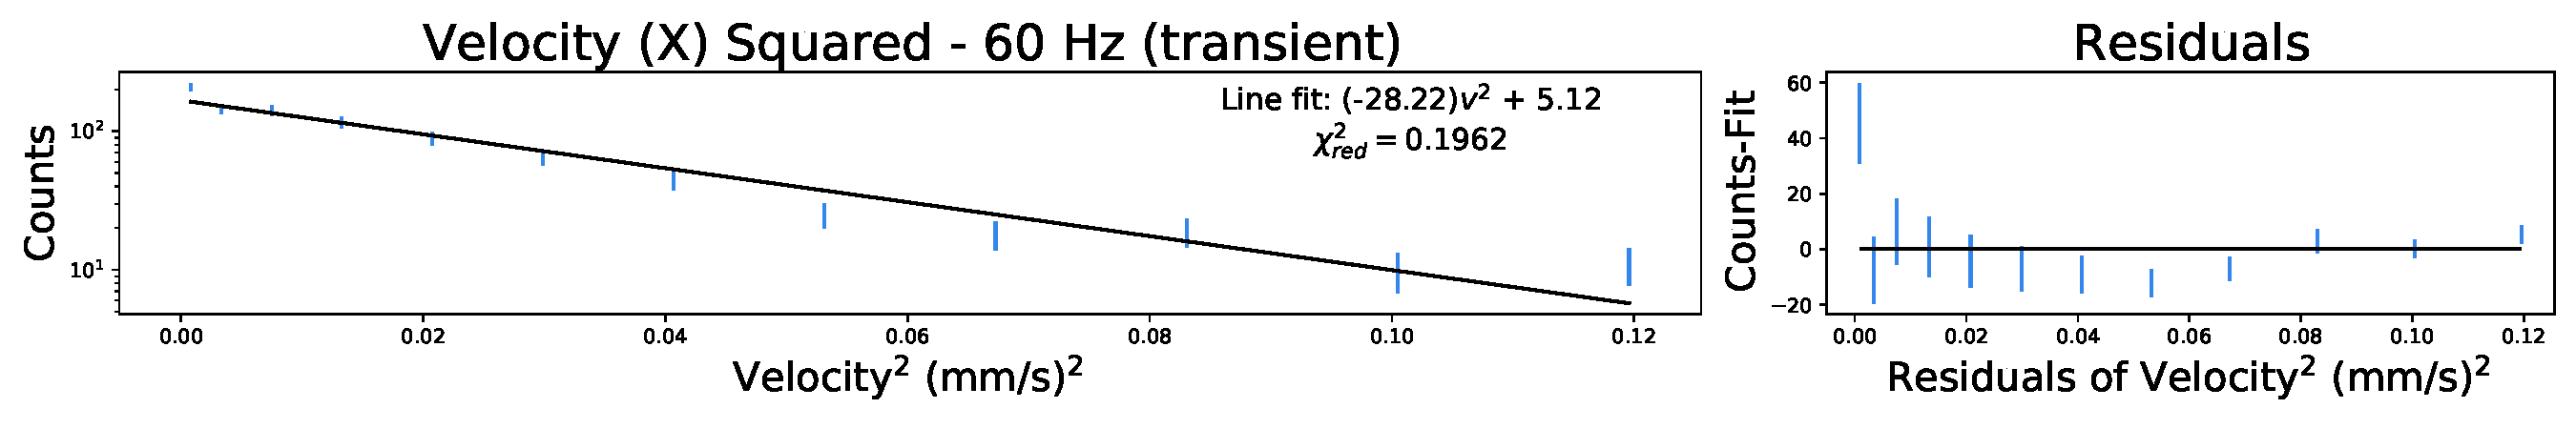
\includegraphics[width=\textwidth]{data_02_x_vel.pdf}
	\caption{}
    \label{fig:02_x_vel}
    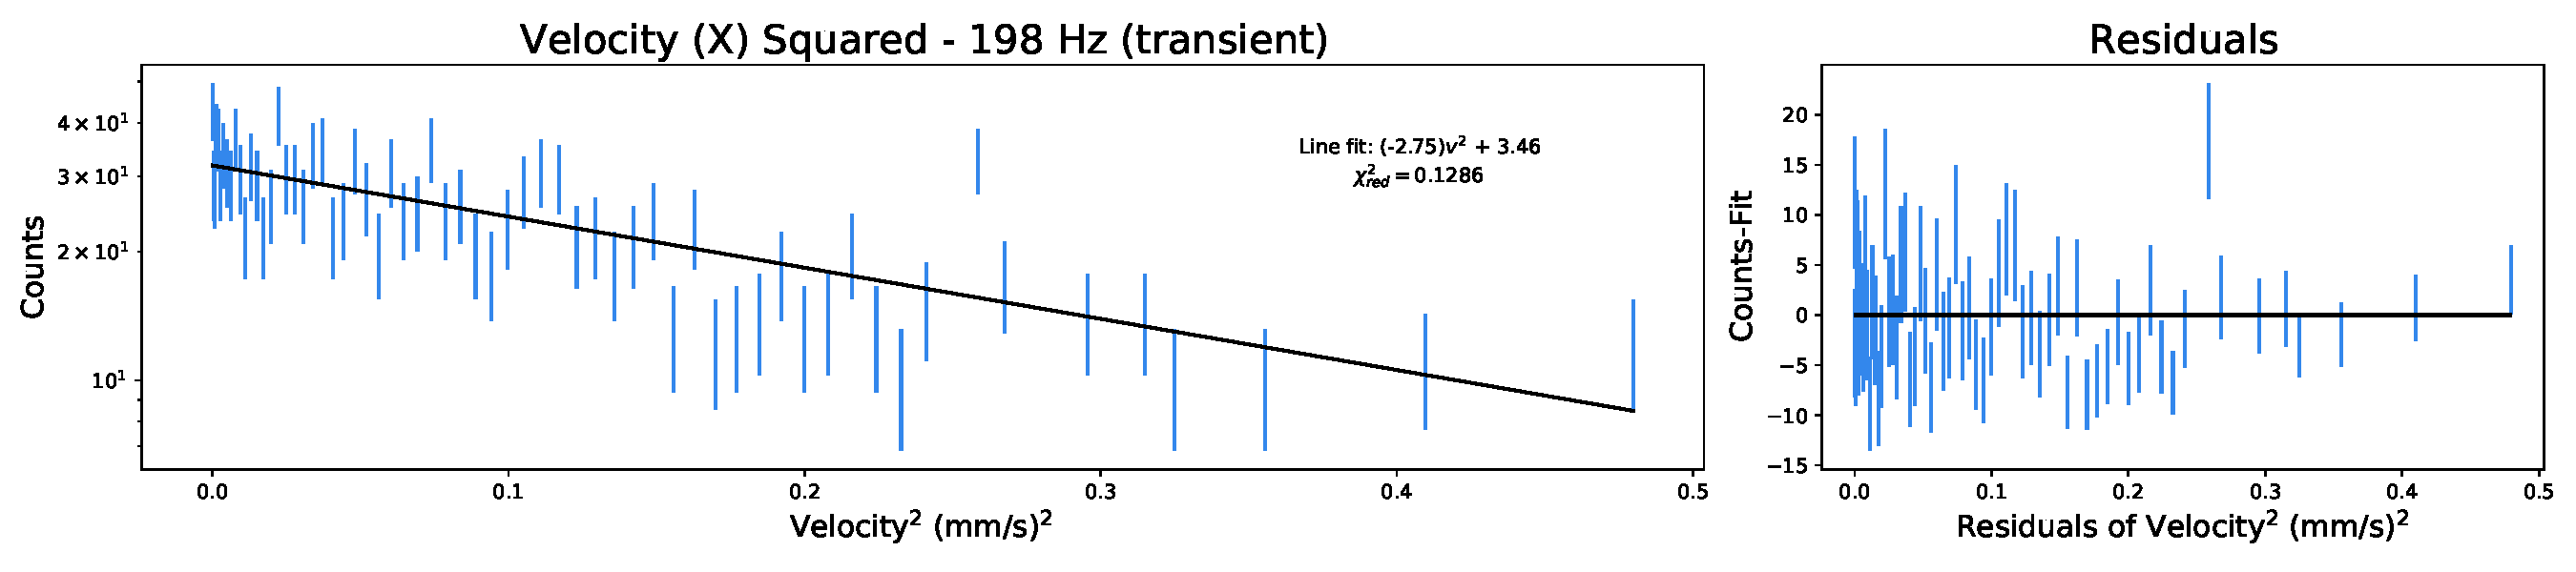
\includegraphics[width=\textwidth]{data_05_x_vel.pdf}
	\caption{}
    \label{fig:05_x_vel}
\end{figure}

\subsection{Calculating Mass}
%% Give the calculated mass, for all of them - provide source of error bar

\subsection{Coulomb Crystal}
%% Give the pics of crystal and analysis that a recording gave. 

%-----------------------------------------------------------------------


\section{Discussion and Conclusions}


%-----------------------------------------------------------------------

\vskip 0.2in
\bibliography{lab04}


\end{document}
